\chapter{Measurement of $\xsecDDbar$ near $\psipp$}
\label{ch:cross_section}


\section{Form Factors}
\label{sec:form_factors}

In Eq. \ref{eq:form_factor}, we assume the $\psip$ resonant contribution is negligible in the energy range of our measurements, so the only major resonant contribution is from the $\psipp$:
\beq
F_D(W) = F_D^{\text{NR}}(W) + F^{\psipp}_D(W) \, e^{i \phi^{\psipp} }.
\eeq

\noindent
Currently, there is no definitive model for the non-resonant term, so we use two alternative parameterizations for this.
The first is a simple exponential model:
\beq
\label{eq:exp_model}
F_D^{NR} = \FNR \, \exp ( -q_D^2 / \aNR^2 ),
\eeq

\noindent 
where both $\FNR$ and $\aNR$ are parameters determined through fitting. 
The second treatment implements a Vector Dominance Model (VDM).
This assumes the interference effects are due to the $\psip$ mediating $\DDbar$ production above threshold,
\beq
\label{eq:vdm_model}
F_D^{NR}(W) = F_D^{\psip}(W) + F_0,
\eeq

\noindent
and that the effective properties of the $\psip$ are similar to those of the $\psipp$.
The real constant $F_0$ represents the potential effect of higher resonances, like the $\psi(4040)$.
The first term is similar to Eq. \ref{eq:breit_wigner}, but with a modification to the total width:
\beq
\label{eq:Gamma_psip}
\Gpsip(W) = \left( \frac{M^{\psip}}{W} \right) \left[ \frac{ z_{\DO \aDO}(W) \, d_{\DO \aDO}(W) + z_{\Dp \Dm}(W) \, d_{\Dp \Dm}(W) }{ z_{\DO \aDO}(M^{\psi''}) \, d_{\DO \aDO}(M^{\psi''}) + z_{\Dp \Dm}(M^{\psi''}) \, d_{\Dp \Dm}(M^{\psi''}) } \right] \Gpsip(M).
\eeq

\noindent
Without this modification, the mass of the $\psip$ would be below the $\DDbar$ threshold, and thus, the vanishing $z_{\DDbar}$ terms would cause a singularity in the width.
Therefore, we use the mass of the $\psipp$ in its place to estimate the effects in this region.
While it may behave like the total width in Eq. \ref{eq:Gamma_psip}, the true the physical meaning of the parameter $\Gpsip(W)$ is uncertain.
For the radii in Eq. \ref{eq:blatt_weisskopf}, however, the values used are distinct for each meson: $R_{\psip} = \SI{0.75}{\fm}$ and $R_{\psipp} = \SI{1.00}{\fm}$.


\section{Data and Monte Carlo Samples}
\label{sec:samples}

\subsection{Data Samples}
\label{ssec:data_samples}

This analysis primarily uses scan data produced by BEPCII and collected by BESIII in 2010 over an energy range of \SIrange{3.643}{3.890}{\GeV}.
These data are partitioned into 35 center-of-mass energy ($\Ecm$) bins of variable size over a range of \SIrange{3.735}{3.870}{\GeV}.
The range was chosen to be above the $\DO\aDO$ threshold (\SI{3.730}{\GeV}) and below the $D^{*0}\aDO$ threshold (\SI{3.872}{\GeV}).
This range includes bins which are below the threshold for $\Dp \Dm$ (\SI{3.739}{\GeV}), with production beginning in the fourth bin.

Additionally, there are three higher statistics points used for comparison.
These include an `On-Peak $\psipp$' sample of \SI{2.93}{\invfb} at $\Ecm = \SI{3.773}{\GeV}$, an `$XYZ$-scan' sample of \SI{50.54}{\invpb} at $\Ecm = \SI{3.810}{\GeV}$, and an `$R$-scan' sample of \SI{7.95}{\invpb} at $\Ecm = \SI{3.850}{\GeV}$.
The first of these was analyzed by Derrick Toth with a separate procedure using double-tag reconstruction (both $\D$ and $\aD$ in a single event).
The other two samples were analyzed using the same procedure as for the scan data (See \Cref{sec:signal,sec:efficiency,sec:fitting}).
None of these points are used to determine the final results, as the differences between samples introduce additional systematics which overshadow any statistical improvement.
However, these provide useful comparisons at important energy points along the cross section shape.


\subsection{Luminosity Calculation}
\label{ssec:luminosity}

The integrated luminosity for each run is calculated following the procedure described in Ref. \cite{ref:Hafner:2015}.
For each run, \num{1.4e6} $\bhabha (\gamma)$ events were generated using Babayaga 3.5.
We then select events with only two (oppositely) charged tracks, satisfying the event selection criteria $V_{xy} < 1$ cm, $|V_z| < 5$ cm, and $|\cos\theta| < 0.8$.
After this, we accept only tracks that satisfy $E_{\text{EMC}} > 0.73 \times \Ebeam$ (cuts on $\ee \rightarrow \mu^+ \mu^- (\gamma)$ events) and $p > 0.93 \times \Ebeam$ (cuts on $\ee \rightarrow \gamma \jpsi, \; \jpsi \rightarrow \ee$ events).
Applying these cuts to both data and MC identically, we use the resulting number of events found in the MC divided by the total generated to determine the efficiency $(\epsilon_{MC})$.
From this, and using the cross section provided by the generator $(\sigma_{BB})$, we can take the events found in data $(N_{\text{data}})$ to determine the integrated luminosity $(\lum)$ of each run:
\beq
\lum = \frac{N_{\text{data}}}{\sigma_{BB} ~ \epsilon_{MC}}
\eeq
The integrated luminosity for each bin is shown in \Cref{tab:luminosity}.
The total luminosity for the data used is \SI{70.05 \pm 0.03}{\invpb}, where the error listed is statistical.

\begin{table}%[h]
\centering
\renewcommand\arraystretch{1.0}
\begin{tabular}{r c l}
\hline
Bin & $\Ecm$ Range [\si{\GeV}] & $\lum$ [\si{\invpb}] \\
\hline
 0 & 3.735 - 3.736 & 0.3357(21) \\ 
 1 & 3.736 - 3.737 & 0.4940(25) \\ 
 2 & 3.737 - 3.744 & 0.3310(21) \\ 
 3 & 3.744 - 3.746 & 0.9626(35) \\ 
 4 & 3.746 - 3.748 & 1.4260(43) \\ 
 5 & 3.748 - 3.750 & 2.2782(54) \\ 
 6 & 3.750 - 3.752 & 2.9970(63) \\ 
 7 & 3.752 - 3.754 & 3.3362(66) \\ 
 8 & 3.754 - 3.755 & 3.4380(67) \\ 
 9 & 3.755 - 3.758 & 3.8841(71) \\ 
10 & 3.758 - 3.761 & 4.4496(76) \\ 
11 & 3.761 - 3.764 & 4.4984(77) \\ 
12 & 3.764 - 3.767 & 3.2856(66) \\ 
13 & 3.767 - 3.770 & 2.4478(57) \\ 
14 & 3.770 - 3.773 & 2.0184(52) \\ 
15 & 3.773 - 3.776 & 1.8294(49) \\ 
16 & 3.776 - 3.779 & 1.8252(49) \\ 
17 & 3.779 - 3.782 & 1.9547(51) \\
18 & 3.782 - 3.785 & 2.1555(53) \\
19 & 3.785 - 3.788 & 2.5510(58) \\
20 & 3.788 - 3.792 & 2.8330(61) \\
21 & 3.792 - 3.796 & 3.5342(69) \\
22 & 3.796 - 3.800 & 4.0536(73) \\
23 & 3.800 - 3.803 & 3.9381(73) \\
24 & 3.803 - 3.806 & 2.7087(60) \\
25 & 3.806 - 3.809 & 1.7671(49) \\
26 & 3.809 - 3.812 & 1.2619(41) \\
27 & 3.812 - 3.815 & 0.9019(35) \\
28 & 3.815 - 3.823 & 0.6846(30) \\
29 & 3.823 - 3.830 & 0.4016(23) \\
30 & 3.830 - 3.839 & 0.2851(20) \\
31 & 3.839 - 3.847 & 0.2804(20) \\
32 & 3.847 - 3.855 & 0.2774(19) \\
33 & 3.855 - 3.863 & 0.3192(21) \\
34 & 3.863 - 3.870 & 0.3001(20) \\
\hline
\end{tabular}
\caption{Measured luminosities for each energy bin.}{The uncertainties listed are statistical errors from the data selection, as uncertainties from the MC statistics are negligible.}
\label{tab:luminosity}
\end{table}


\subsection{Monte Carlo Generation}
\label{ssec:monte_carlo}

To compare to the scan data sample, several Monte Carlo (MC) samples were produced.
For the main signal determination, samples of generic $\DO \aDO$ from $\psipp$ and generic $\Dp \Dm$ from $\psipp$ were generated with \num{e5} events per run.
In addition, $100\times$ data-size samples were produced for $\qqbar$, $\tautau$, radiative return to $\jpsi$ (denoted $\gamma \jpsi$), and radiative return to $\psip$ (denoted $\gamma \psi'$).
Each of these samples was generated at the University of Minnesota in July of 2014 using BOSS 6.6.4.p02.
The $\DO \aDO$, $\Dp \Dm$, $\qqbar$, and $\tautau$ states were generated using KKMC, while the $\gamma \jpsi$ and $\gamma \psi'$ were generated with BesEvtGen.
All except $\qqbar$ were then decayed with BesEvtGen.
The total numbers of events in each sample can be found in \Cref{tab:mc_samples}.

\begin{table}[h]
\centering
\renewcommand\arraystretch{1.0}
\begin{tabular}{c c}
\hline
Sample & Number of Events \\
\hline
$\psipp \rightarrow \DO \aDO$ & \num{1.660e7} \\
$\psipp \rightarrow \Dp \Dm$  & \num{1.620e7} \\
$\qqbar$                      & \num{8.916e7} \\
$\gamma \jpsi$                & \num{7.307e6} \\
$\gamma \psi'$                & \num{2.457e7} \\
$\tautau$                     & \num{2.164e7} \\
Data                          & \num{4.844e8} \\
\hline
\end{tabular}
\caption{Number of events contained in each generated sample and the scan data.}
\label{tab:mc_samples}
\end{table}

In general, all MC samples were generated based off communal decay card information used within BESIII. 
However, the $\DDbar$ samples were generated by implementing the Born-level cross section shape from the final fit into KKMC.
This procedure was repeated over four iterations in order to provide a more data-driven basis for the ISR corrections.
The effects of this process are examined in \Cref{sec:systematics}.


\subsection{Software Packages}
\label{ssec:software}


\section{Signal Determination}
\label{sec:signal}

We measure the yields of both $\DO \aDO$ and $\Dp \Dm$ events with two-dimensional fits to $\DeltaE$ and $\mbc$.
MC samples are partitioned into the following four groups: proper $D$-tags ($N_{\DDbar}$), misreconstructed $D$-tags ($N_{\text{misrec}}$), continuum ($N_{\qqbar}$), and other ($N_\text{other}$).
The first two groups are obtained using truth information from the $\DDbar$ samples, while the last group is a combination of the $\tautau$, $\gamma \jpsi$, and $\gamma \psi'$ samples.
These groups are fitted to data using the RooFit package to perform a negative log-likelihood minimization for each energy bin ($E_i$) separately for both $\DO$ and $\Dp$.
For each fit, the four MC sample groups are used to construct 2D ($\DeltaE$ vs. $\mbc$) PDF functions that are fitted against the corresponding data histograms.
The proper $\DDbar$ shape is treated as signal, and its integral after fitting $(N_{D})$ is used for determining the signal yields and cross sections.
An example fit is shown in Fig. \ref{fig:example_fit}, while the complete set of these plots can be found in \Cref{app:D0_signal_fits,app:Dp_signal_fits}.

\begin{figure}[h]
\centering
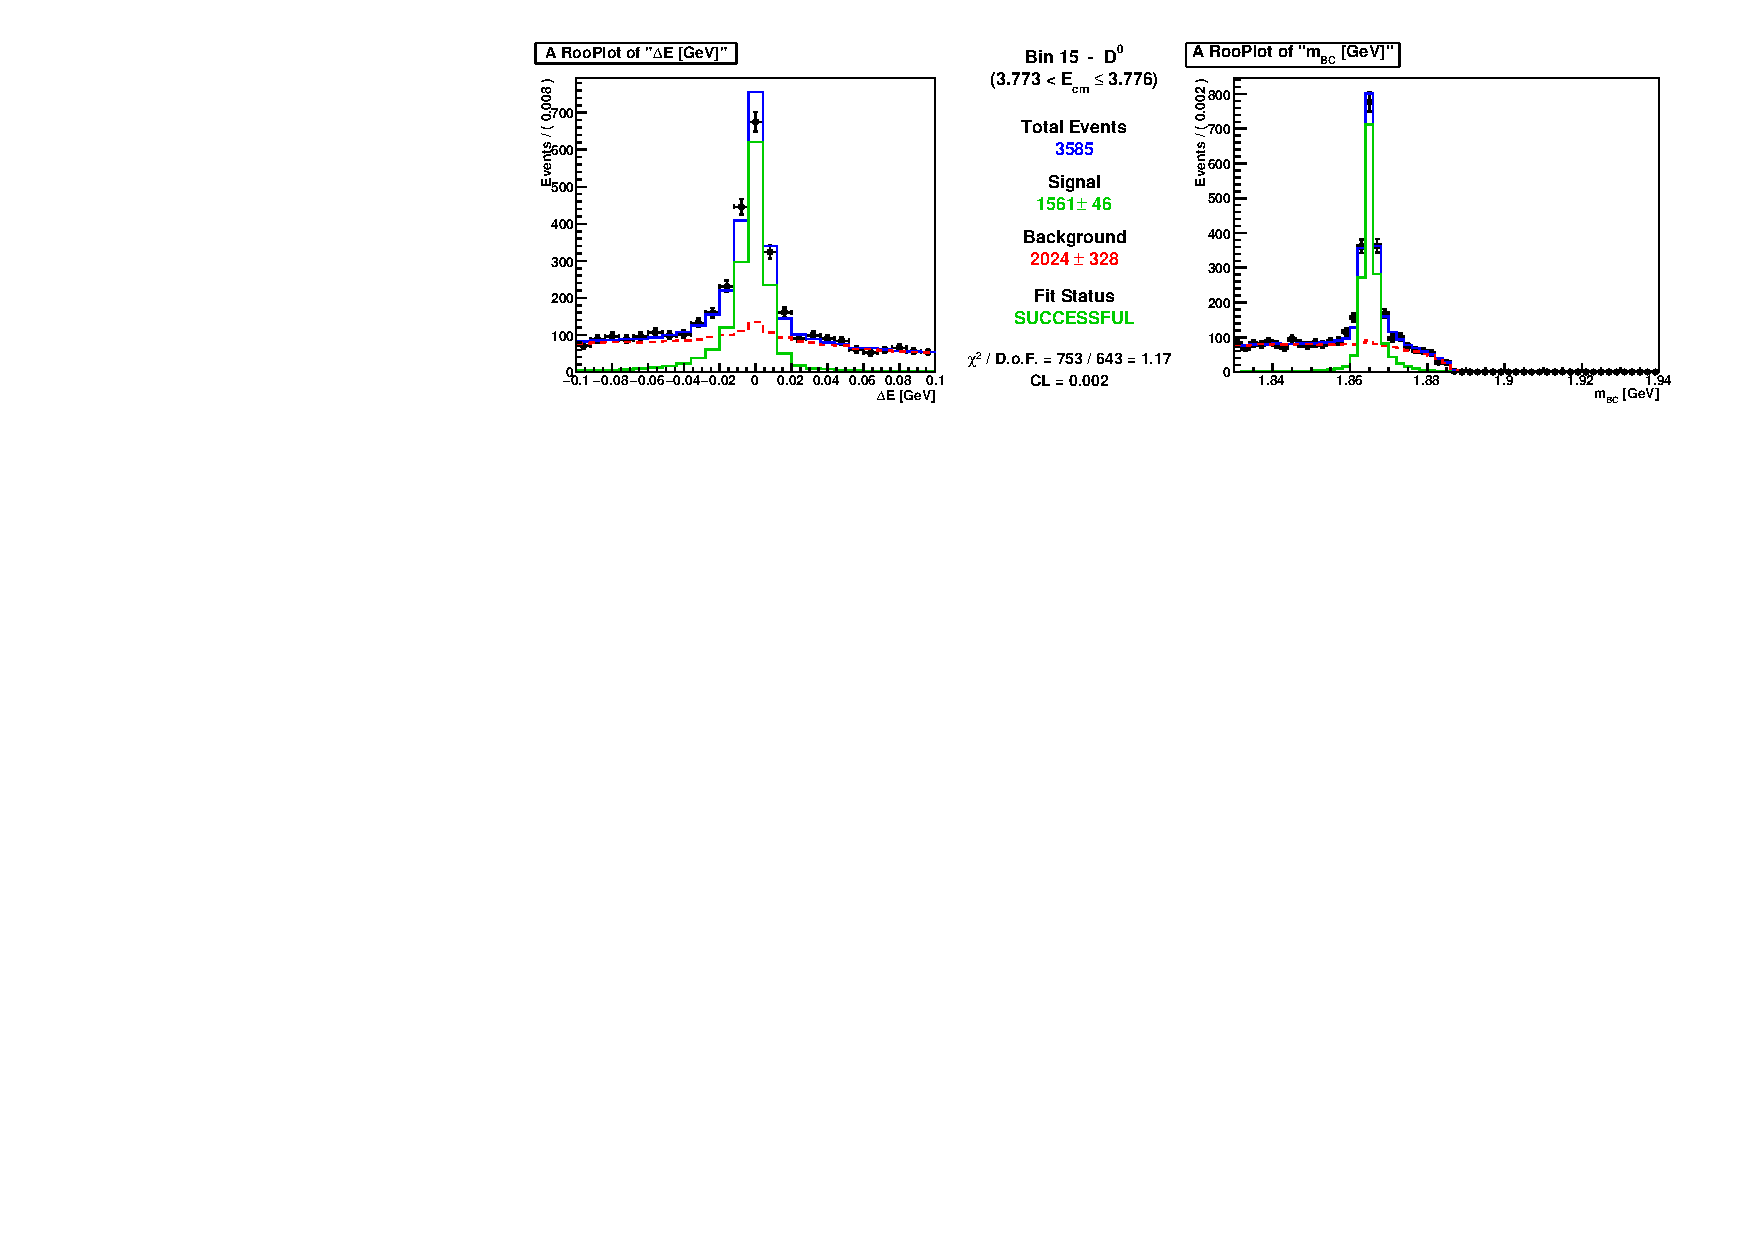
\includegraphics[scale=0.75]{figures/plots/fit_results/D0_bin_15.pdf}
\caption{An example 2D signal fit.}{The covers $\DO$ events in the region $\SI{3.773}{\GeV} < \Ecm \leq \SI{3.776}{\GeV}$.
The data points (black) are fitted by the total MC shape (blue), which is the sum of the signal (green) and background (red) components.}
\label{fig:example_fit}
\end{figure}


\section{Efficiency Correction}
\label{sec:efficiency}

In addition to the parameters gathered by \DTagAlg, truth information was taken from the generic $\DDbar$ samples in order to determine the mode-by-mode reconstruction efficiency.
To be deemed proper, a reconstruction must pass not only the standard $\Dtag$ cuts, but also match the generator information for the event.
This process removes peaking backgrounds from modes with similar constituents.
The total number of proper $\Dtag$ reconstructions is then divided by the number of $\D$ particles generated for each mode, and the mode-by-mode efficiencies are weighted by the PDG branching ratios \cite{ref:Olive:2014} to determine the overall efficiency ($\epsilon_{\D}$) for each of $\DO$ and $\Dp$:
\beq
\label{eq:DDbar_eff}
\epsilon_{D} = \sum_i \epsilon_i \, \mathcal{B}_i = \sum_i \left( \frac{ N_{i \text{ proper}} }{ N_{i \text{ generated}} } \right) \mathcal{B}_i.
\eeq
Each $\DO$ efficiency also includes the corresponding DCSD terms for its decay (See \Cref{sec:d_tagging}).

To determine the cross section at each point, this procedure was applied separately for each energy bin.
The total number of proper and generated particles for each energy bin are shown in \Cref{tab:DTag_eff_D0} for $\DO$ and \Cref{tab:DTag_eff_Dp_p1,tab:DTag_eff_Dp_p2} for $\Dp$.
The efficiencies for $\Dp$ and $\DO$ were also calculated across the total sample, and are shown for each mode in \Cref{tab:DTag_eff} and \Cref{fig:D_eff_by_mode}.
Each energy bin's total efficiency for both $\DO$ and $\Dp$ is shown in \Cref{tab:DTag_eff_E_bin}.

\begin{table}
\renewcommand\arraystretch{1.0}
\centering
\begin{tabular}{c|R{1.5cm}R{1.5cm}|R{1.5cm}R{1.5cm}|R{1.5cm}R{1.5cm}}
\hline
Bin & \multicolumn{2}{c|}{$\DOmodeA$} & \multicolumn{2}{c|}{$\DOmodeB$} & \multicolumn{2}{c}{$\DOmodeC$} \\
& $\Nprop$ & $\Ngen$ & $\Nprop$ & $\Ngen$ & $\Nprop$ & $\Ngen$ \\
\hline
 0 &   5519  &   7658  &  10757  &  27894  &   6927  &  16948  \\
 1 &  11203  &  15778  &  21753  &  56203  &  13704  &  33428  \\
 2 &   5470  &   7686  &  10761  &  27725  &   6929  &  16962  \\
 3 &  10987  &  15550  &  21357  &  55223  &  13639  &  33704  \\
 4 &  16311  &  23268  &  31913  &  83399  &  19997  &  50031  \\
 5 &  27586  &  38880  &  53505  & 138886  &  33927  &  83498  \\
 6 &  49416  &  69908  &  95785  & 250493  &  60813  & 150614  \\
 7 &  43530  &  62064  &  85248  & 222230  &  54013  & 134237  \\
 8 &  49056  &  70191  &  95402  & 250020  &  61035  & 150852  \\
 9 &  38764  &  54791  &  75237  & 194185  &  48307  & 116868  \\
10 &  55219  &  77765  & 107785  & 277958  &  69525  & 167368  \\
11 &  55412  &  78328  & 108229  & 278765  &  68944  & 167385  \\
12 &  38502  &  54639  &  75111  & 194082  &  48743  & 117181  \\
13 &  32802  &  46683  &  64440  & 166338  &  41593  & 100543  \\
14 &  21886  &  30983  &  43041  & 111230  &  27326  &  66506  \\
15 &  21849  &  31151  &  42979  & 110746  &  27406  &  66800  \\
16 &  16534  &  23429  &  31906  &  83165  &  20645  &  50035  \\
17 &  21963  &  31442  &  42724  & 110981  &  27807  &  67080  \\
18 &  27328  &  38791  &  53480  & 139055  &  34434  &  83489  \\
19 &  27019  &  38726  &  53396  & 139091  &  34605  &  83915  \\
20 &  38332  &  54586  &  75296  & 194835  &  47966  & 117143  \\
21 &  38032  &  54321  &  74841  & 195177  &  47764  & 117511  \\
22 &  43289  &  62110  &  84373  & 222186  &  53400  & 133871  \\
23 &  48974  &  70058  &  93686  & 249998  &  58965  & 150580  \\
24 &  32426  &  46536  &  62154  & 166927  &  38264  &  99797  \\
25 &  27022  &  38674  &  51590  & 138723  &  31748  &  83715  \\
26 &  16588  &  23491  &  30978  &  83656  &  19168  &  50246  \\
27 &  10832  &  15519  &  20060  &  55573  &  12281  &  33523  \\
28 &  10651  &  15284  &  20306  &  55439  &  12505  &  33815  \\
29 &  10980  &  15661  &  20233  &  55701  &  12405  &  33649  \\
30 &   5398  &   7822  &   9954  &  27637  &   6060  &  16711  \\
31 &   5425  &   7804  &  10010  &  27618  &   6156  &  16729  \\
32 &   5439  &   7830  &  10009  &  27799  &   5988  &  16695  \\
33 &  10659  &  15442  &  20070  &  55385  &  12282  &  33515  \\
34 &  10615  &  15443  &  19910  &  55573  &  12345  &  33592  \\
\hline
\end{tabular}
\caption{Number of proper and generated particles for $\DO$.}
{The mode-by-mode numbers of particles used in the efficiency calculations for $\DOmodeA, \DOmodeB,$ and $\DOmodeC$.}
\label{tab:DTag_eff_D0}
\end{table}


\begin{table}
\renewcommand\arraystretch{1.0}
\centering
\begin{tabular}{c|R{1.25cm}R{1.25cm}|R{1.25cm}R{1.25cm}|R{1.25cm}R{1.25cm}}
\hline
Bin & \multicolumn{2}{c|}{$\DpmodeA$} & \multicolumn{2}{c|}{$\DpmodeB$} & \multicolumn{2}{c}{$\DpmodeC$} \\
& $\Nprop$ & $\Ngen$ & $\Nprop$ & $\Ngen$ & $\Nprop$ & $\Ngen$ \\
\hline
 3 &  20022  &  37668  &   6600  &  24160  &   2272  &   5902  \\
 4 &  30234  &  56234  &  10010  &  36416  &   3431  &   8931  \\
 5 &  50966  &  93874  &  16855  &  60686  &   5750  &  14833  \\
 6 &  91414  & 169401  &  29807  & 109330  &  10199  &  26677  \\
 7 &  81267  & 150434  &  26528  &  96948  &   9060  &  23797  \\
 8 &  90448  & 168761  &  30206  & 109641  &  10233  &  26927  \\
 9 &  71896  & 131281  &  23901  &  85264  &   8167  &  20918  \\
10 & 103179  & 187949  &  34092  & 121352  &  11695  &  29969  \\
11 & 103605  & 188336  &  34331  & 122120  &  11672  &  29828  \\
12 &  72921  & 132064  &  23962  &  84947  &   8199  &  20937  \\
13 &  62056  & 112433  &  20547  &  72991  &   7021  &  17781  \\
14 &  41328  &  75280  &  13636  &  48338  &   4739  &  11979  \\
15 &  41441  &  75211  &  13640  &  48504  &   4613  &  11861  \\
16 &  31212  &  56487  &  10309  &  36655  &   3513  &   8982  \\
17 &  41621  &  75045  &  13881  &  49145  &   4680  &  12048  \\
18 &  51909  &  94077  &  16905  &  60819  &   5769  &  14879  \\
19 &  52042  &  94156  &  17035  &  60618  &   5885  &  14977  \\
20 &  72086  & 131300  &  23647  &  84907  &   8286  &  21035  \\
21 &  72509  & 131694  &  23555  &  84570  &   8029  &  20806  \\
22 &  82597  & 150805  &  26792  &  96787  &   9334  &  23503  \\
23 &  92228  & 169069  &  29808  & 109702  &  10559  &  26985  \\
24 &  61616  & 113123  &  19611  &  73321  &   6985  &  18018  \\
25 &  50613  &  93767  &  16383  &  60811  &   5712  &  14759  \\
26 &  30736  &  56653  &   9583  &  36280  &   3614  &   9245  \\
27 &  20427  &  37582  &   6456  &  24186  &   2250  &   5811  \\
28 &  20295  &  37687  &   6536  &  24289  &   2214  &   5811  \\
29 &  20393  &  37337  &   6489  &  24201  &   2466  &   6167  \\
30 &  10309  &  18737  &   3128  &  12099  &   1159  &   3003  \\
31 &  10345  &  18895  &   3216  &  12023  &   1120  &   2946  \\
32 &  10142  &  18893  &   3213  &  12066  &   1168  &   3020  \\
33 &  20265  &  37114  &   6374  &  24194  &   2330  &   5967  \\
34 &  20311  &  37337  &   6362  &  24378  &   2326  &   6057  \\
\hline
\end{tabular}
\caption{Number of proper and generated particles for $\Dp$ (part 1).}
{The mode-by-mode numbers of particles used in the efficiency calculations for $\DpmodeA, \DpmodeB,$ and $\DpmodeC$.}
\label{tab:DTag_eff_Dp_p1}
\end{table}


\begin{table}
\renewcommand\arraystretch{1.0}
\centering
\begin{tabular}{c|R{1.25cm}R{1.25cm}|R{1.25cm}R{1.25cm}|R{1.25cm}R{1.25cm}}
\hline
Bin & \multicolumn{2}{c|}{$\DpmodeD$} & \multicolumn{2}{c|}{$\DpmodeE$} & \multicolumn{2}{c}{$\DpmodeF$} \\
& $\Nprop$ & $\Ngen$ & $\Nprop$ & $\Ngen$ & $\Nprop$ & $\Ngen$ \\
\hline
 3 &   5578  &  27502  &   3414  &  14899  &   1698  &   3980  \\
 4 &   8468  &  41353  &   4999  &  22340  &   2485  &   5867  \\
 5 &  14556  &  69102  &   8309  &  37104  &   4344  &   9959  \\
 6 &  25432  & 124123  &  14807  &  66943  &   7430  &  17744  \\
 7 &  22850  & 110296  &  13319  &  60059  &   6723  &  15843  \\
 8 &  25820  & 124151  &  15057  &  66954  &   7478  &  17655  \\
 9 &  20373  &  96362  &  11898  &  52068  &   6093  &  13955  \\
10 &  29030  & 138372  &  17076  &  74519  &   8425  &  19594  \\
11 &  29195  & 137508  &  17221  &  74539  &   8534  &  19799  \\
12 &  20216  &  96603  &  12006  &  52123  &   5985  &  13833  \\
13 &  17507  &  82589  &  10228  &  44534  &   5111  &  11746  \\
14 &  11705  &  54998  &   6839  &  29643  &   3429  &   7891  \\
15 &  11602  &  55245  &   6810  &  29770  &   3461  &   7989  \\
16 &   8763  &  41572  &   4963  &  22250  &   2564  &   5876  \\
17 &  11651  &  55576  &   6953  &  29754  &   3341  &   7827  \\
18 &  14509  &  68677  &   8617  &  37138  &   4235  &   9867  \\
19 &  14565  &  68864  &   8466  &  36828  &   4361  &   9826  \\
20 &  20572  &  97073  &  12192  &  52476  &   6187  &  13850  \\
21 &  20411  &  96827  &  11748  &  52152  &   5898  &  13671  \\
22 &  23090  & 109958  &  13325  &  59244  &   6906  &  15913  \\
23 &  25746  & 124249  &  14667  &  66799  &   7601  &  17652  \\
24 &  17179  &  82921  &   9571  &  44714  &   4994  &  11729  \\
25 &  14120  &  69390  &   7922  &  37132  &   4165  &   9905  \\
26 &   8380  &  41424  &   4794  &  22343  &   2562  &   5908  \\
27 &   5593  &  27680  &   3072  &  14738  &   1694  &   3935  \\
28 &   5627  &  27587  &   3151  &  14791  &   1657  &   3859  \\
29 &   5677  &  27727  &   3118  &  14862  &   1700  &   3924  \\
30 &   2863  &  13875  &   1604  &   7514  &    849  &   2003  \\
31 &   2733  &  13650  &   1554  &   7495  &    828  &   1971  \\
32 &   2808  &  13903  &   1491  &   7273  &    876  &   2005  \\
33 &   5572  &  27708  &   3168  &  14898  &   1659  &   3890  \\
34 &   5627  &  27755  &   3095  &  14821  &   1692  &   3962  \\
\hline
\end{tabular}
\caption{Number of proper and generated particles for $\Dp$ (part 2).}
{The mode-by-mode numbers of particles used in the efficiency calculations for $\DpmodeD, \DpmodeE,$ and $\DpmodeF$.}
\label{tab:DTag_eff_Dp_p2}
\end{table}


\begin{table}[h]
\centering
\begin{tabular}{l c c}
\hline
Decay Mode ($i$) & PDG $\mathcal{B}_i$ [\%] & MC Efficiency $\epsilon_i$ \\
\hline
$\DOmodeA$ & \pp 3.89 $\pm$ 0.05 & 0.70226(74) \\ 
$\DOmodeB$ &    13.93 $\pm$ 0.50 & 0.38190(29) \\ 
$\DOmodeC$ & \pp 8.11 $\pm$ 0.20 & 0.40277(38) \\ 
\hline
\multicolumn{3}{c}{$\epsilon_{\DO}$ = (11.320 $\pm$ 0.213)\%} \\
\hline
$\DpmodeA$ & \pp 9.13 $\pm$ 0.19 & 0.54699(42)\pp \\
$\DpmodeB$ & \pp 5.99 $\pm$ 0.18 & 0.27570(38)\pp \\
$\DpmodeC$ & \pp 1.47 $\pm$ 0.07 & 0.38972(89)\pp \\
$\DpmodeD$ & \pp 6.99 $\pm$ 0.27 & 0.20864(31)\pp \\
$\DpmodeE$ & \pp 3.12 $\pm$ 0.11 & 0.22540(43)\pp \\
$\DpmodeF$ & \pp 0.95 $\pm$ 0.03 & 0.43199(116)   \\
\hline
\multicolumn{3}{c}{$\epsilon_{\Dp}$ = (9.792 $\pm$ 0.134)\%} \\[1pt]
\hline
\end{tabular}
\caption{Mode-by-mode reconstruction efficiencies for $\DO$ and $\Dp$.}
{The values shown are over the entire data sample, while calculations for the cross sections use the values of each energy point individually.}
\label{tab:DTag_eff}
\end{table}


\begin{figure}[h]
\centering
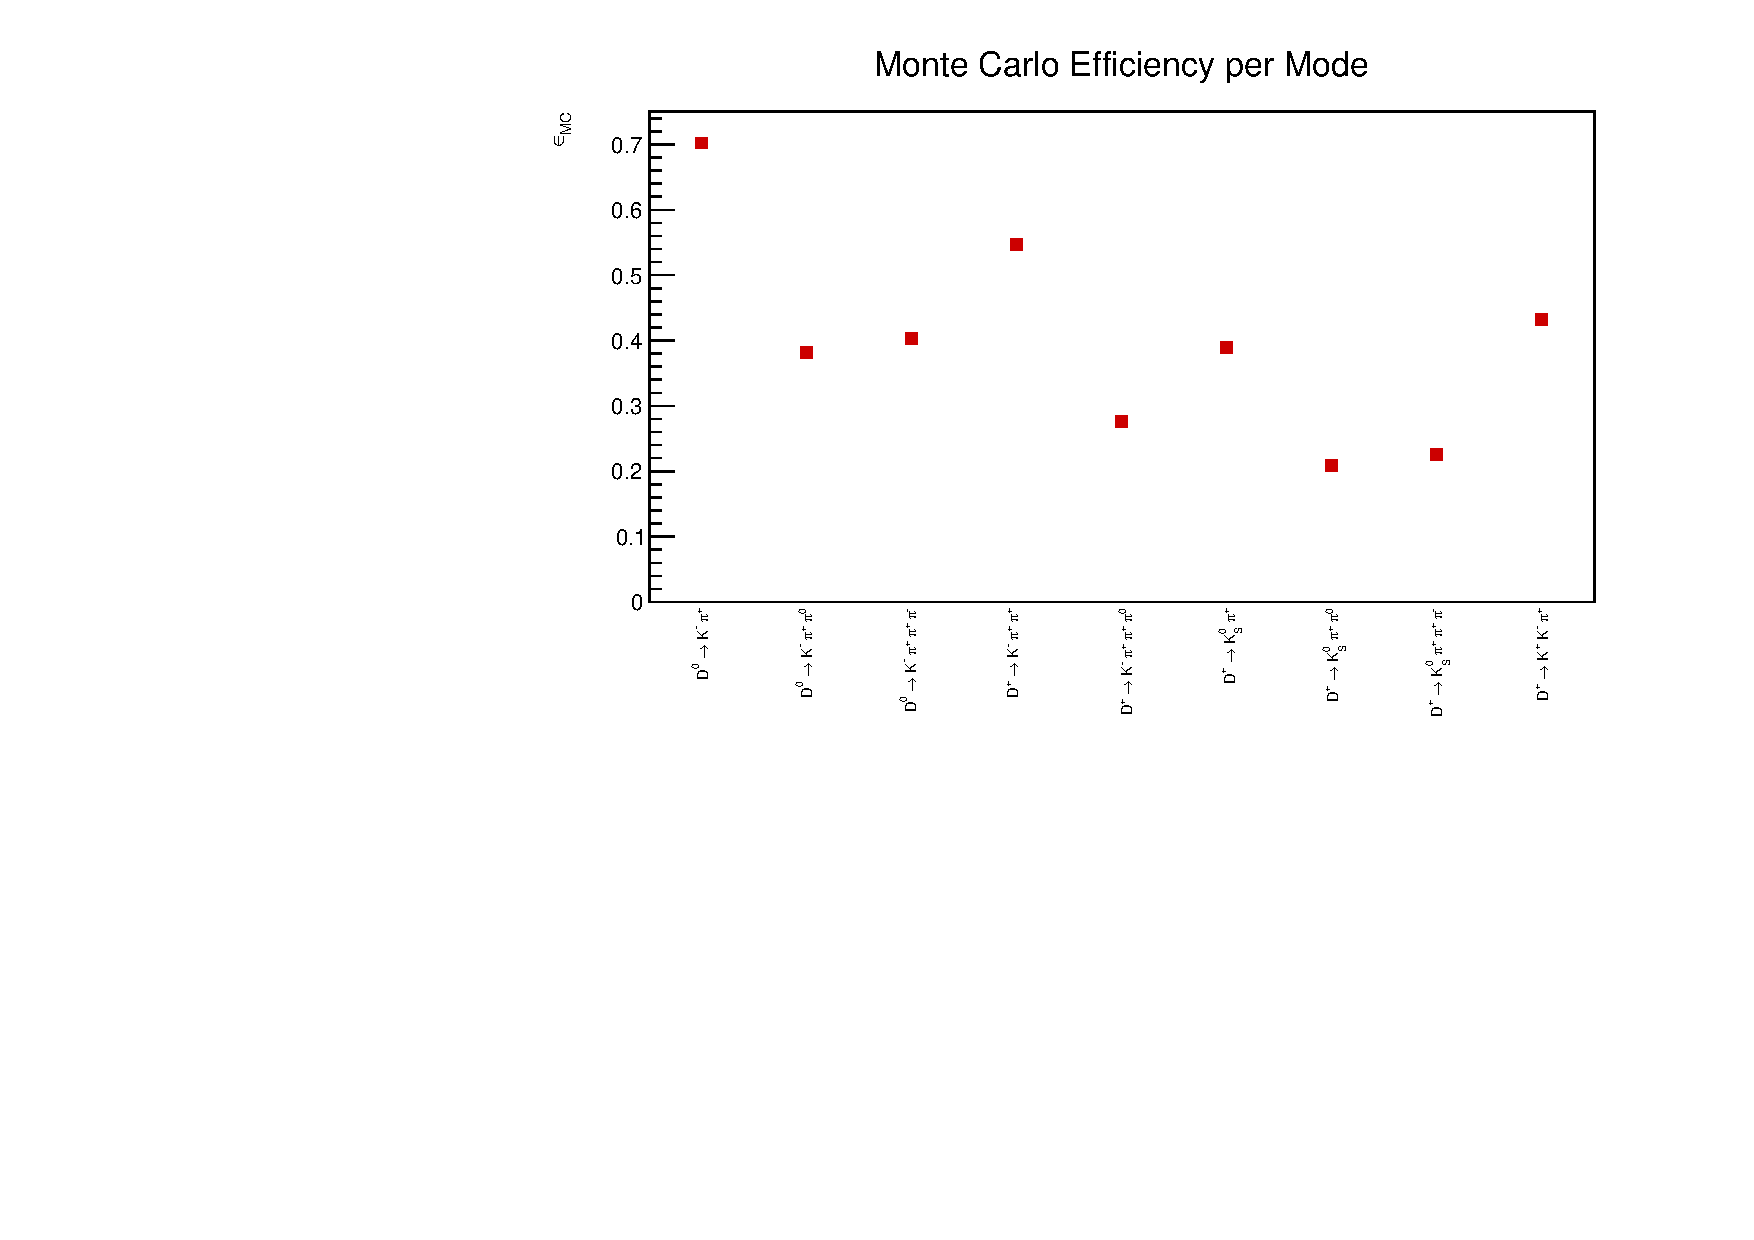
\includegraphics[scale=0.8]{figures/plots/D_eff_by_mode.pdf}
\caption{Mode-by-mode MC efficiencies for $\DO$ and $\Dp$.}
{The error bars are negligible on the scale shown.}
\label{fig:D_eff_by_mode}
\end{figure}


\begin{table}
\centering
\renewcommand\arraystretch{1.0}
\begin{tabular}{c C{3cm} C{3cm}}
\hline
$E_{\text{bin}}$ & $\epsilon_{\DO}$ & $\epsilon_{\Dp}$ \\
\hline
 0 & 0.1149 $\pm$ 0.0023 & -                   \\ 
 1 & 0.1148 $\pm$ 0.0022 & -                   \\ 
 2 & 0.1149 $\pm$ 0.0023 & -                   \\ 
 3 & 0.1142 $\pm$ 0.0022 & 0.0959 $\pm$ 0.0014 \\ 
 4 & 0.1130 $\pm$ 0.0022 & 0.0965 $\pm$ 0.0014 \\ 
 5 & 0.1142 $\pm$ 0.0022 & 0.0978 $\pm$ 0.0014 \\ 
 6 & 0.1135 $\pm$ 0.0021 & 0.0964 $\pm$ 0.0013 \\ 
 7 & 0.1134 $\pm$ 0.0021 & 0.0968 $\pm$ 0.0013 \\ 
 8 & 0.1132 $\pm$ 0.0021 & 0.0966 $\pm$ 0.0013 \\ 
 9 & 0.1150 $\pm$ 0.0022 & 0.0986 $\pm$ 0.0014 \\ 
10 & 0.1153 $\pm$ 0.0022 & 0.0986 $\pm$ 0.0014 \\ 
11 & 0.1150 $\pm$ 0.0022 & 0.0990 $\pm$ 0.0014 \\ 
12 & 0.1151 $\pm$ 0.0022 & 0.0990 $\pm$ 0.0014 \\ 
13 & 0.1149 $\pm$ 0.0022 & 0.0992 $\pm$ 0.0014 \\ 
14 & 0.1147 $\pm$ 0.0022 & 0.0991 $\pm$ 0.0014 \\ 
15 & 0.1146 $\pm$ 0.0022 & 0.0988 $\pm$ 0.0014 \\ 
16 & 0.1144 $\pm$ 0.0022 & 0.0989 $\pm$ 0.0014 \\ 
17 & 0.1144 $\pm$ 0.0022 & 0.0993 $\pm$ 0.0014 \\
18 & 0.1144 $\pm$ 0.0022 & 0.0988 $\pm$ 0.0014 \\
19 & 0.1141 $\pm$ 0.0022 & 0.0993 $\pm$ 0.0014 \\
20 & 0.1144 $\pm$ 0.0022 & 0.0989 $\pm$ 0.0014 \\
21 & 0.1136 $\pm$ 0.0022 & 0.0985 $\pm$ 0.0014 \\
22 & 0.1124 $\pm$ 0.0021 & 0.0983 $\pm$ 0.0014 \\
23 & 0.1112 $\pm$ 0.0021 & 0.0973 $\pm$ 0.0014 \\
24 & 0.1101 $\pm$ 0.0021 & 0.0967 $\pm$ 0.0014 \\
25 & 0.1098 $\pm$ 0.0021 & 0.0960 $\pm$ 0.0014 \\
26 & 0.1100 $\pm$ 0.0021 & 0.0961 $\pm$ 0.0014 \\
27 & 0.1072 $\pm$ 0.0021 & 0.0960 $\pm$ 0.0014 \\
28 & 0.1081 $\pm$ 0.0021 & 0.0959 $\pm$ 0.0014 \\
29 & 0.1078 $\pm$ 0.0021 & 0.0968 $\pm$ 0.0014 \\
30 & 0.1064 $\pm$ 0.0021 & 0.0965 $\pm$ 0.0015 \\
31 & 0.1074 $\pm$ 0.0021 & 0.0961 $\pm$ 0.0015 \\
32 & 0.1063 $\pm$ 0.0021 & 0.0953 $\pm$ 0.0015 \\
33 & 0.1071 $\pm$ 0.0021 & 0.0961 $\pm$ 0.0014 \\
34 & 0.1065 $\pm$ 0.0021 & 0.0957 $\pm$ 0.0014 \\
\hline
\end{tabular}
\caption{The overall reconstruction efficiency of $\DO$ and $\Dp$ for each energy bin.}
{These values are used to calculate the corresponding cross sections at each energy point.  The listed errors are statistical only.}
\label{tab:DTag_eff_E_bin}
\end{table}


\subsection{$\sCP$ Violation Correction}
\label{ssec:cp_correction}

Due to $\sCP$ violation in the $\DO \aDO$ system, each of the neutral decay modes must be corrected to account for quantum correlations.
This is done by applying scaling factors to the efficiency for each of the three modes used in reconstruction.
The corrections are parameterized for each mode ($m$) by the following form \cite{ref:Asner:2008}:
\beq
\label{eq:qc}
\alpha_{\DO \rightarrow m} = 1 + r_m^2 + 2 \times y \times r_m \times R_m \times \cos(\delta_m).
\eeq
Here, $r_m$ and $\delta_m$ represent the relative magnitudes and phases between the Cabbibo-favored and doubly-Cabbibo-suppressed modes, respectively, while the factor of $R_m$ represents a coherence factor characterizing the variation of $\delta_m$ over phase space.
Note, there is no such variation for a two-body decay (like $\DOmodeA$), so $R_{\DOmodeA} = 1$.
The value of $y$ represents the difference in total width components of the $\DO \aDO$ system, $y = (\Gamma_2 - \Gamma_1) / (\Gamma_2 + \Gamma_1)$, where 1 and 2 represent the $\sCP$-odd and $\sCP$-even states, respectively.

The mode-dependent values for these factors are listed in \Cref{tab:qc_factors}.
These are taken from the $CPV$-allowed values in \cite{ref:HFAG:2015} for $\DOmodeA$, and from \cite{ref:Evans:2016} for $\DOmodeB$ and $\DOmodeC$.
The value of $y = 0.0066^{+0.0007}_{-0.0010}$ is also from \cite{ref:HFAG:2015}, and is the same for all modes.
After applying each of the mode-dependent corrections, the efficiency for the full sample changes from $\epsilon_{\DO} = (11.320 \pm 0.213)\%$ to $\epsilon_{\DO} = (11.352 \pm 0.213)\%$, and similarly for the efficiencies of each $\Ecm$ bin.

\begin{table}[h]
\renewcommand\arraystretch{1.0}
\begin{tabular}{l|r@{$\;\pm\;$}l r@{~}l r@{~}l|r@{~}l}
\hline 
\multicolumn{1}{c|}{Mode}  & \multicolumn{2}{c}{$r_m$} & \multicolumn{2}{c}{$R_m$} & \multicolumn{2}{c|}{$\delta_m$ [\si{^\circ}]} & \multicolumn{2}{c}{$\alpha_m$} \\
\hline
$\DOmodeA$ & 0.0591 & 0.0063 & \multicolumn{2}{c}{1}         &  11.8 & $^{+\;\pp 9.5}_{-\;14.7}$ & 1.00426 & $ \pm\; 0.00083$             \\
$\DOmodeB$ & 0.0447 & 0.0012 & 0.81 & $\pm\; 0.06$           &  18   & $^{+\;   14  }_{-\;15  }$ & 1.00248 & $ \pm\; 0.00014$             \\
$\DOmodeC$ & 0.0549 & 0.0006 & 0.43 & $^{+\;0.17}_{-\;0.13}$ & -52   & $^{+\;   28  }_{-\;17  }$ & 1.00270 & $^{+\;0.00014}_{-\;0.00012}$ \\
\hline 
\end{tabular}
\caption{The quantum correlated factors for the $\DO$ modes.}
\label{tab:qc_factors}
\end{table}


\section{Fitting Procedure}
\label{sec:fitting}

After applying the correction in \Cref{ssec:cp_correction}, the efficiency values (\Cref{tab:DTag_eff_E_bin}) were combined with the luminosity (\Cref{tab:luminosity}) and the signal values from each 2D fit (\Cref{tab:xsec_rc_data}) to determine the cross section at each energy point.  Since each $\psipp$ produces a $\DDbar$ pair, a factor of 2 is included to avoid double counting:
\beq
\label{eq:xsec_rc_data}
\sigma_{\DDbar}^{RC}(E_i) = \frac{ N_D(E_i) }{ 2 \, \epsilon_D(E_i) \, \mathcal{L}(E_i) }.
\eeq
The resulting cross section values for $\DO$ and $\Dp$ are also listed in \Cref{tab:xsec_rc_data}, and shown in \Cref{fig:xsec_rc_data}.


\begin{table}%[h]
\centering
\begin{tabular}{c r@{$\;\pm\;$}l r@{$\;\pm\;$}l r@{$\;\pm\;$}l r@{$\;\pm\;$}l}
\hline
$E_{\text{mid}}$ & \multicolumn{2}{c}{$N_{\DO \aDO}$} & \multicolumn{2}{c}{$\sigma^{RC}_{\DO \aDO}$ [\si{\nb}]} & \multicolumn{2}{c}{$N_{\Dp \Dm}$}  & \multicolumn{2}{c}{$\sigma^{RC}_{\Dp \Dm}$ [\si{\nb}]} \\
\hline
3.7355 &   12 &  5 & 0.155 & 0.065 & \multicolumn{2}{c}{-} & \multicolumn{2}{c}{-} \\ 
3.7364 &   24 &  7 & 0.212 & 0.066 & \multicolumn{2}{c}{-} & \multicolumn{2}{c}{-} \\ 
3.7377 &   15 &  5 & 0.204 & 0.069 & \multicolumn{2}{c}{-} & \multicolumn{2}{c}{-} \\ 
3.7447 &  166 & 15 & 0.761 & 0.072 &   27 &  6 & 0.147 & 0.038 \\ 
3.7464 &  266 & 20 & 0.823 & 0.064 &   98 & 12 & 0.361 & 0.046 \\  
3.7485 &  508 & 27 & 0.970 & 0.056 &  199 & 17 & 0.446 & 0.040 \\ 
3.7503 &  825 & 34 & 1.210 & 0.055 &  321 & 22 & 0.555 & 0.039 \\ 
3.7525 & 1012 & 38 & 1.334 & 0.057 &  479 & 27 & 0.743 & 0.043 \\ 
3.7541 & 1143 & 41 & 1.462 & 0.059 &  510 & 28 & 0.767 & 0.044 \\ 
3.7556 & 1454 & 45 & 1.622 & 0.059 &  680 & 32 & 0.887 & 0.044 \\ 
3.7586 & 1993 & 53 & 1.940 & 0.064 & 1036 & 39 & 1.177 & 0.048 \\ 
3.7616 & 2388 & 58 & 2.303 & 0.071 & 1323 & 44 & 1.493 & 0.054 \\ 
3.7646 & 2016 & 53 & 2.662 & 0.086 & 1224 & 42 & 1.884 & 0.070 \\ 
3.7675 & 1719 & 48 & 3.051 & 0.104 & 1050 & 38 & 2.174 & 0.086 \\ 
3.7705 & 1578 & 46 & 3.391 & 0.119 & 1044 & 38 & 2.610 & 0.103 \\ 
3.7735 & 1561 & 46 & 3.708 & 0.131 & 1116 & 39 & 3.086 & 0.118 \\ 
3.7765 & 1543 & 45 & 3.673 & 0.130 & 1108 & 39 & 3.058 & 0.118 \\ 
3.7795 & 1522 & 46 & 3.372 & 0.121 & 1001 & 38 & 2.579 & 0.105 \\
3.7826 & 1398 & 44 & 2.826 & 0.106 &  957 & 38 & 2.248 & 0.095 \\
3.7855 & 1140 & 41 & 1.948 & 0.080 &  806 & 36 & 1.589 & 0.075 \\
3.7885 &  848 & 38 & 1.310 & 0.064 &  645 & 34 & 1.147 & 0.064 \\
3.7925 &  725 & 37 & 0.903 & 0.050 &  480 & 30 & 0.688 & 0.045 \\
3.7964 &  514 & 35 & 0.561 & 0.040 &  321 & 31 & 0.403 & 0.040 \\
3.8005 &  354 & 31 & 0.404 & 0.037 &  182 & 28 & 0.238 & 0.037 \\
3.8036 &  194 & 23 & 0.324 & 0.039 &  117 & 22 & 0.223 & 0.043 \\
3.8065 &  125 & 19 & 0.323 & 0.050 &   95 & 16 & 0.280 & 0.050 \\
3.8095 &   57 & 13 & 0.206 & 0.048 &   33 & 13 & 0.138 & 0.055 \\
3.8124 &   11 &  9 & 0.056 & 0.050 &   29 & 11 & 0.168 & 0.065 \\
3.8157 &    6 &  7 & 0.046 & 0.050 &    8 &  8 & 0.067 & 0.062 \\
3.8237 &   11 &  7 & 0.128 & 0.081 &   15 &  8 & 0.196 & 0.108 \\
3.8315 &    7 &  5 & 0.118 & 0.086 &    2 &  6 & 0.039 & 0.114 \\
3.8397 &   15 &  6 & 0.254 & 0.108 &   12 &  6 & 0.239 & 0.119 \\
3.8475 &   14 &  6 & 0.250 & 0.109 &    9 &  6 & 0.172 & 0.121 \\
3.8556 &   26 &  8 & 0.377 & 0.117 &   16 &  6 & 0.269 & 0.108 \\
3.8636 &   15 &  6 & 0.236 & 0.099 &    7 &  5 & 0.138 & 0.095 \\
\hline
\end{tabular} 
\caption{The $\DDbar$ cross section at each $\Ecm$ point.}
{The number of data events observed in each $\Ecm$ bin are also shown.
The uncertainties on the cross sections are statistical only and come from the signal fitting ($N_D$), PDG values (\Cref{tab:DTag_eff}), and MC reconstruction efficiency (\Cref{tab:DTag_eff_E_bin}).
The values for $N_{\DO \aDO}$ and $N_{\Dp \Dm}$ are taken from the signal fits shown in \Cref{app:D0_signal_fits,app:Dp_signal_fits}.}
\label{tab:xsec_rc_data}
\end{table}


\begin{figure}[h]
\centering
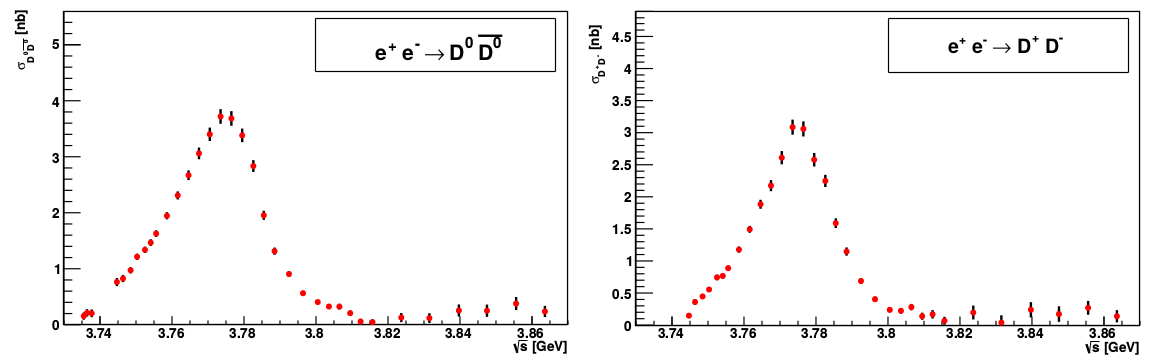
\includegraphics[scale=0.35]{figures/plots/xsec_data.png}
\caption{The measured $\ee \rightarrow \DDbar$ cross sections.}
{The $\DO \aDO$ cross section is shown on the left and $\Dp \Dm$ is shown on the right. }
\label{fig:xsec_rc_data}
\end{figure}


Using the measured $\DDbar$ cross sections, we fit to \Cref{eq:xsec_rc_simp} using each of the form factor choices described in \Cref{sec:form_factors}.
In each case, there are four common fit parameters: $\Mpsipp$, $\Gpsipp$, $\Geepsipp$, and $\Ppsipp$.
These represent the mass, total width, electron partial width, and relative phase to the non-resonant contribution for the $\psipp$, respectively.
This notation for the total width corresponds to $\Gamma(M)$ in \Cref{sec:xsec_derivation}.
Two additional fitting parameters are dependent on which form factor is being used: $F_{NR}$ and $a_{NR}$ for the exponential, or $\Gpsip$ and $F_0$ for the VDM.
For the former, these represent the amplitude and exponent normalization for the non-resonant contribution.
In the latter case, these represent the modified total width for the $\psip$ above resonance (see \Cref{sec:form_factors}) and the constant contribution of resonances above the $\psipp$.
The fitting is done simultaneously for $\DO$ and $\Dp$ with identical parameters using TMinuit with a $\chi^2$ minimization.
The value minimized is the sum of the $\chi^2$ values from each of the $\DO$ and $\Dp$ cross section functions.  
Results for the Exponential and VDM choices are shown in \Cref{fig:exp_results,fig:vdm_results}, respectively.


\begin{figure}[H]
\centering
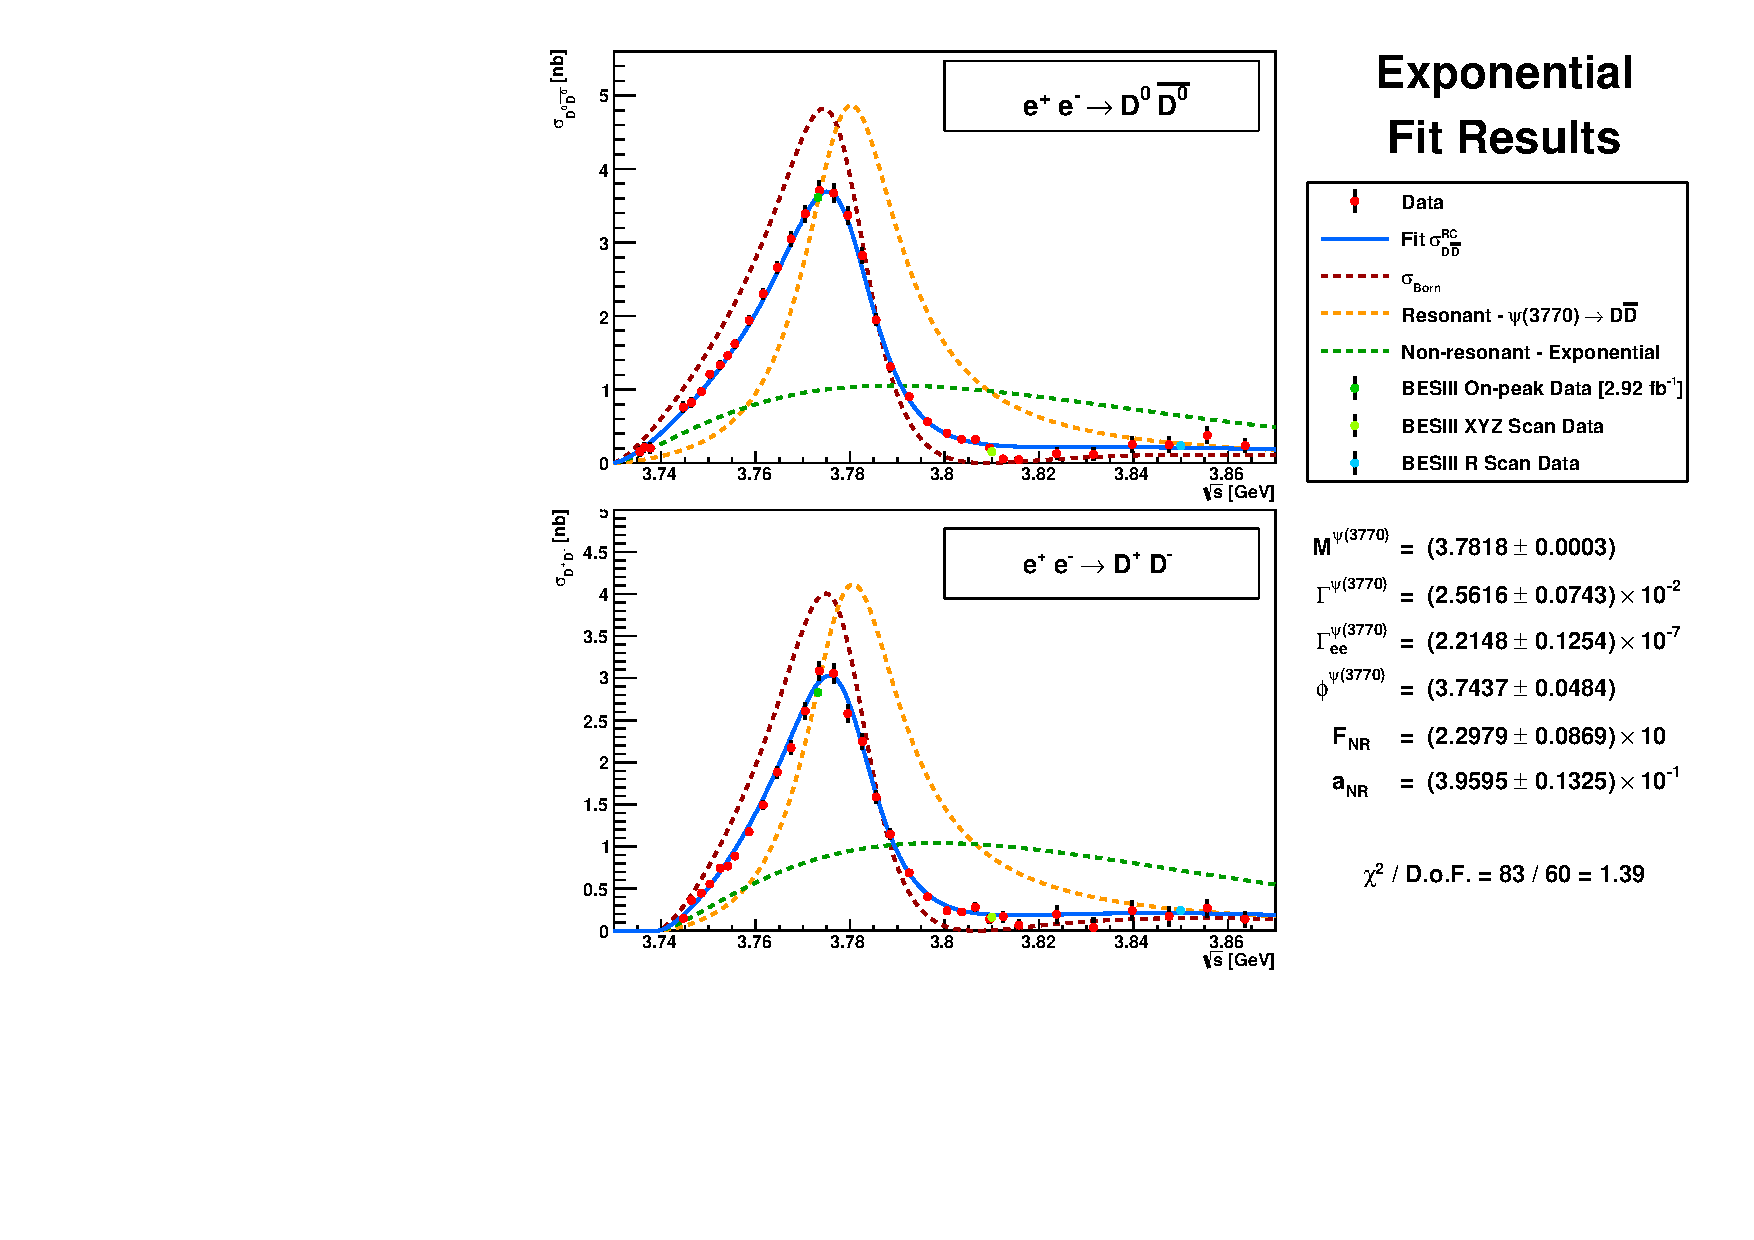
\includegraphics[scale=0.75]{figures/plots/lineshape_exp.pdf}
\caption{The Exponential Model fit results.}
{The results for $\DO$ are shown on the top and the results for $\Dp$ are shown on the bottom. The fit shape (blue) is calculated from \Cref{eq:xsec_rc} using the non-resonant component from \Cref{eq:exp_model}.}
\label{fig:exp_results}
\end{figure}

\begin{figure}%[h]
\centering
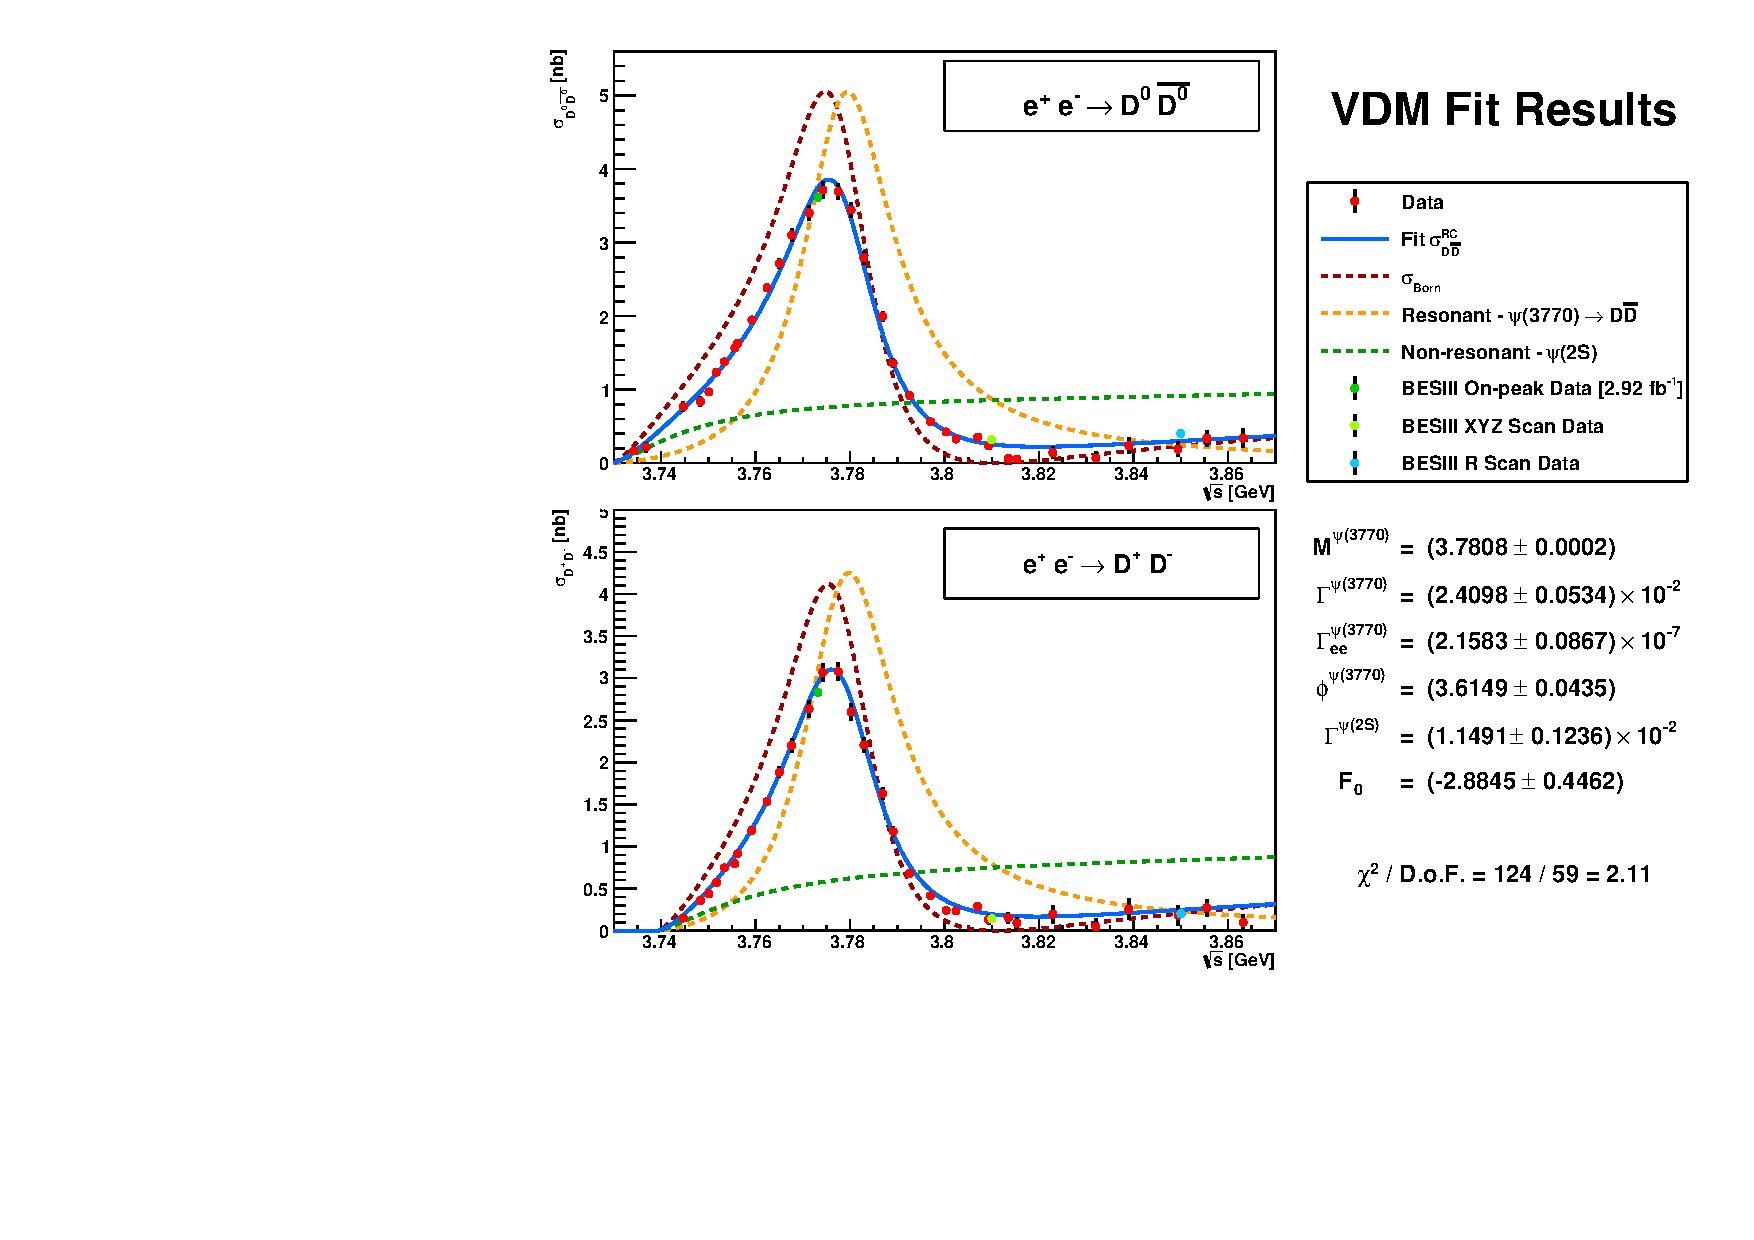
\includegraphics[scale=0.75]{figures/plots/lineshape_vdm.pdf}
\caption{The Vector Dominance Model fit results.}
{The results for $\DO$ are shown on the top and the results for $\Dp$ are shown on the bottom. The fit shape (blue) is calculated from \Cref{eq:xsec_rc} using the non-resonant component from \Cref{eq:vdm_model}.}
\label{fig:vdm_results}
\end{figure}


\subsection{Coulomb Correction}
\label{ssec:coulomb}

In the development of this analysis, it was discovered that the theoretical formulation in \Cref{sec:xsec_derivation} did not lead to a successful fit of the $\DDbar$ cross sections, shown in \Cref{fig:vdm_Coulomb}.
Namely, including the Coulomb effect pulls the $\DO \aDO$ and $\Dp \Dm$ cross sections in opposite directions.
We found the best fits were achieved by altering \Cref{eq:z_Dp} to set the Coulomb factor to 1.
While this disagrees with conventional theoretical wisdom, it is consistent with studies of $\Upsilon(4S) \rightarrow B\overline{B}$ where applying a Coulomb correction for the charged final state also leads to inconsistency with data.

\begin{figure}%[h]
\centering
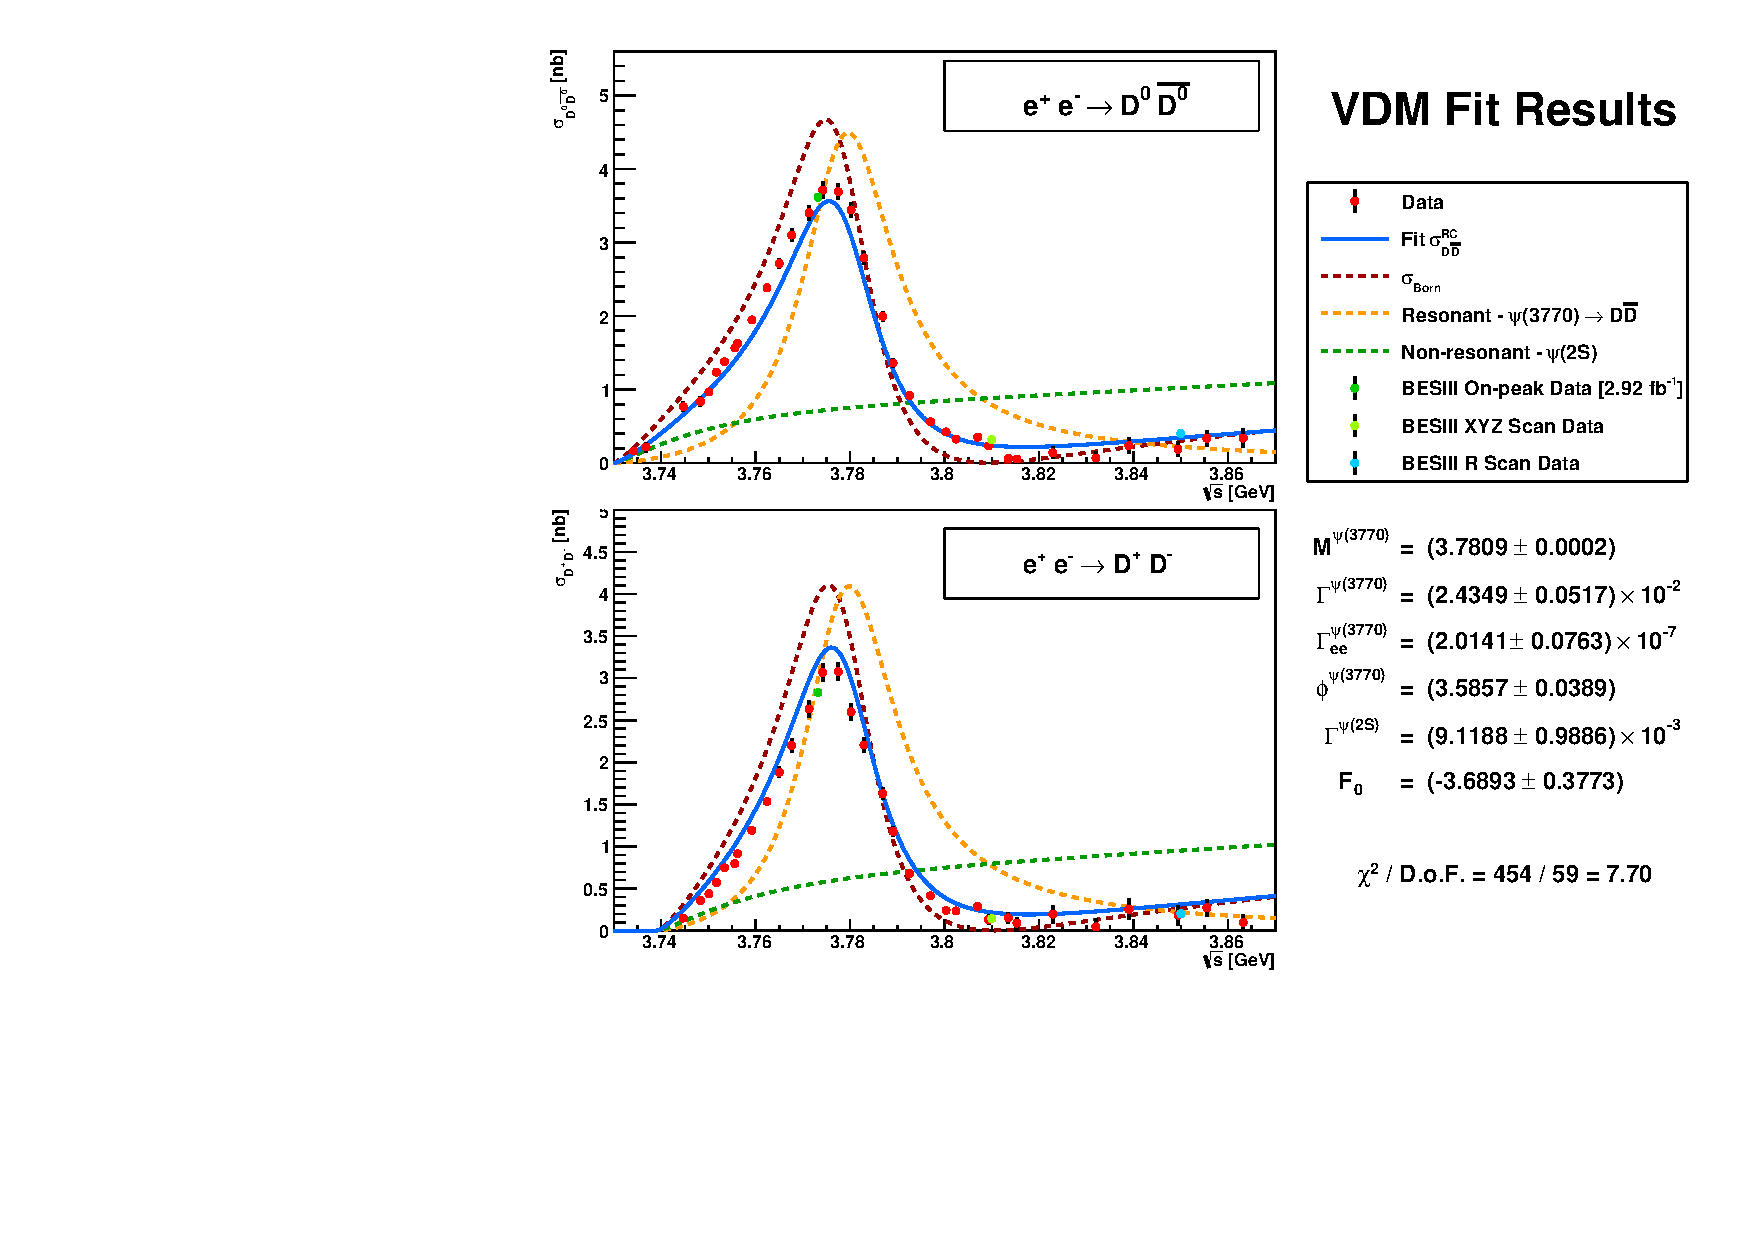
\includegraphics[scale=0.75]{figures/plots/lineshape_vdm_Coulomb.pdf}
\caption{The Vector Dominance Model fit results with Coulomb interactions.}
{The results for $\DO$ are shown on the top and the results for $\Dp$ are shown on the bottom.  Including this factor provides notably worse results than when excluding it (see \Cref{fig:vdm_results}).}
\label{fig:vdm_Coulomb}
\end{figure}

This is most clearly seen in the ratio of $\Dp \Dm$ and $\DO \aDO$ cross sections, shown in \Cref{fig:Coulomb_ratio}, where the `No Coulomb' method sets $\zDD$ in \Cref{eq:xsec_rc_simp,eq:Gamma} to unity, the `Partial Coulomb' sets this factor to unity only for \Cref{eq:xsec_rc_simp}, and the `Full Coulomb' is the default assumption.
Agreement of the measured cross section ratio with the `No Coulomb' calculation is substantially better.
This is also true for the high statistics points measured at the $\psipp$ peak by Derrick Toth \cite{ref:Derrick_memo} (light blue).
As the data tend to follow the `No Coulomb' method, we choose this as our nominal method for the results, presented in \Cref{sec:results}.
However, the interpretation for this behavior is still undetermined.

\begin{figure}%[h]
\centering
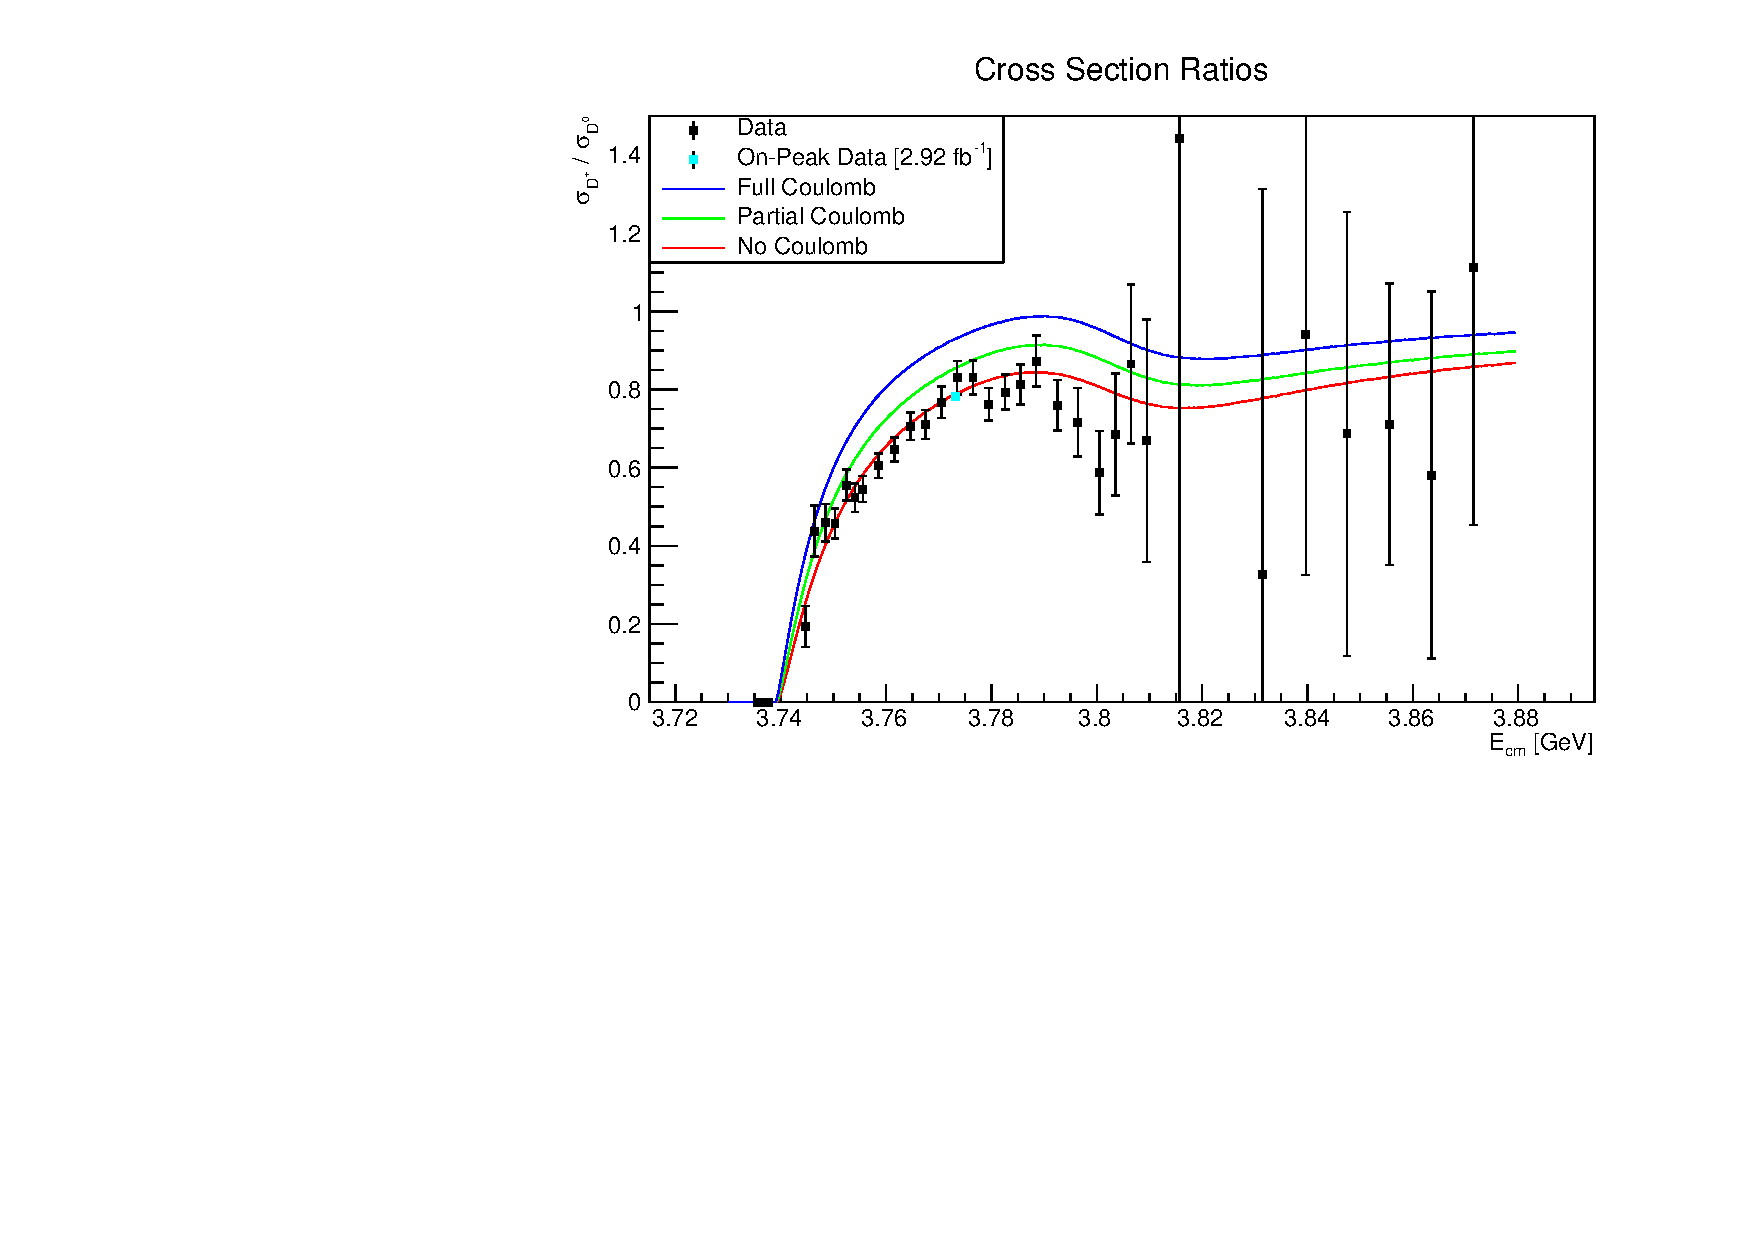
\includegraphics[scale=0.75]{figures/plots/Coulomb_ratio.pdf}
\caption{The ratio of $\Dp$ to $\DO$ cross sections.}
{Several levels of Coulomb interactions are examined.}
\label{fig:Coulomb_ratio}
\end{figure}


\section{Systematics}
\label{sec:systematics}

To assess the systematic uncertainties in our results, we look at a variety of factors.
Many of these affect all BESIII analyses, such as luminosity and tracking.
Others, like the modification to KKMC generation (see \Cref{ssec:monte_carlo}), are specific to this analysis.
The remaining systematics are typically due to less well-known parameters, like the radii used to describe the $\psip$ and $\psipp$ (see \Cref{sec:form_factors}).
Each of these contributions, as well as their total, can be found in \Cref{tab:systematics}. 

Each systematic is obtained by changing a specific aspect, and re-fitting to the altered values using the VDM method.
The uncertainties for each parameter are obtained by taking the difference between this result and the nominal fit (\Cref{fig:vdm_results}).
Generally, each change was done both positively and negatively, and the values used are the largest differences seen between the two changes.
The systematics examined in this analysis are summarized below, where a * denotes aspects which were deemed negligible.


\subsection*{Luminosity}
\label{ssec:sys_luminosity}

A \SI{1}{\%} change was applied to $\lum$ in \Cref{eq:xsec_rc_data}.


\subsection*{$\pipm / \Kpm$ Tracking}
\label{ssec:sys_Kpi_tracking}

A \SI{1.0}{\%} change was applied for each $\pipm$ or $\Kpm$ in a given decay mode.  
The summed contribution for each mode is applied to $\epsilon_m$ in \Cref{eq:DDbar_eff}.


\subsection*{$\piO$ Tracking}
\label{ssec:sys_pi0_tracking}

A \SI{2.0}{\%} change was applied for each $\piO$ in a given decay mode.
The summed contribution for each mode is applied to $\epsilon_m$ in \Cref{eq:DDbar_eff}.


\subsection*{$\Ks$ Tracking}
\label{ssec:sys_Ks_tracking}

A \SI{1.5}{\%} change was applied for each $\Ks$ in a given decay mode.
The summed contribution for each mode is applied to $\epsilon_m$ in \Cref{eq:DDbar_eff}.


\subsection*{Single Tag Fitting}
\label{ssec:sys_single_tag}

A mode-dependent change was applied to $N$ in \Cref{eq:xsec_rc_data}.
Differences from fitting were obtained by Derrick Toth after examining the use of single-Gaussian convolved signal shapes, and are shown in \Cref{tab:sys_single_tag}. 
The changes applied were obtained from the sums of the mode-dependent values averaged over their efficiencies.


\begin{table}[H]
\centering
\renewcommand\arraystretch{1.0}
\begin{tabular}{l|c}
\hline
\multicolumn{1}{c|}{Tag Mode} & Difference (\%) \\
\hline
$\DOmodeA$ & 0.27 \\
$\DOmodeB$ & 0.10 \\
$\DOmodeC$ & 0.47 \\
\hline
\multicolumn{2}{c}{$\DO$ Average: \SI{0.25}{\%}} \\
\hline
$\DpmodeA$ & 0.20 \\
$\DpmodeB$ & 0.00 \\
$\DpmodeC$ & 0.17 \\
$\DpmodeD$ & 0.29 \\
$\DpmodeE$ & 0.17 \\
$\DpmodeF$ & 0.74 \\
\hline
\multicolumn{2}{c}{$\Dp$ Average: \SI{0.20}{\%}} \\
\hline
\end{tabular}
\caption{Single-tag fitting differences by mode.}
{The total $\DO$ and $\Dp$ values are averaged over the efficiencies for each mode.}
\label{tab:sys_single_tag}
\end{table}


\subsection*{KKMC Generation*}
\label{ssec:sys_kkmc}

In generating MC for this analysis, the $\DDbar$ samples used a modified form of KKMC which generates events based off an input Born cross-section shape for the $\psipp$.
However, as this shape is also the final output of the procedure, only an estimation of the results can be used for generation.
To assess the variation from the input shape, we compared the output fit parameters to those used in the generation process.
This process used the Exponential method, and the results are shown in \Cref{tab:KKMC_parameters}.
The numbers listed are from an earlier iteration of the MC than shown in \Cref{sec:fitting}, but the consistency seen is representative of all iterations.
Very little difference is seen in the primary fitting parameters of the $\psipp$.
These similarities show the fit result values converging, even after only a single iteration.
From this, we treat variations due to MC iteration as negligible.

\begin{table}[h!]
\centering
\renewcommand\arraystretch{1.0}
\begin{tabular}{l c|r@{ $\pm$ }l r@{ $\pm$ }l|c}
\hline
\multicolumn{2}{c}{Parameter} & \multicolumn{2}{c}{KKMC Input} & \multicolumn{2}{c}{Fit Results} & Difference \\
\hline
$\Mpsipp$       & [\si{\GeV}] &   3.7815 &  0.0003 &   3.7814 &  0.0003 & 0.0001 \\
$\Gpsipp$       & [\si{\MeV}] &  24.887  &  0.686  &  24.839  &  0.681  & 0.048  \\
$\GeepsipptoDD$ & [\si{\eV}]  & 217.55   & 11.18   & 214.65   & 11.10   & 2.90   \\
$\Ppsipp$       &             &   3.6374 &  0.0513 &   3.6375 &  0.0518 & 0.0001 \\
$\FNR$          &             &  21.394  &  1.866  &  20.147  &  1.765  & 0.992  \\
$\aNR$          &             &  -1.6202 &  0.5271 &  -1.5265 &  0.5119 & 0.0937 \\
\hline
\end{tabular} 
\caption{Comparison of input and output fit parameters.}
{The MC generation is done using the Exponential form factor model as an input Born cross section to generate $\DDbar$ events using KKMC.}
\label{tab:KKMC_parameters}
\end{table}


\subsection*{ConExc Generation*}
\label{ssec:sys_conexc}

To compare to the MC samples generated by KKMC, we also generated alternative MC samples of $\DDbar$ using the ConExc generator.
This process used an input Born level shape identical to that used in the final iteration produced with KKMC.
Each of the background samples used (such as $\qqbar$ and $\tautau$) were the same as in the nominal procedure.
The cross section results using the VDM model are shown in \Cref{fig:ConExc}, and provide $\psipp$ fit parameters within the statistical errors of the nominal method, as seen in \Cref{fig:vdm_results}.
From this, we treat variations due to the MC generator as negligible.

\begin{figure}
\centering
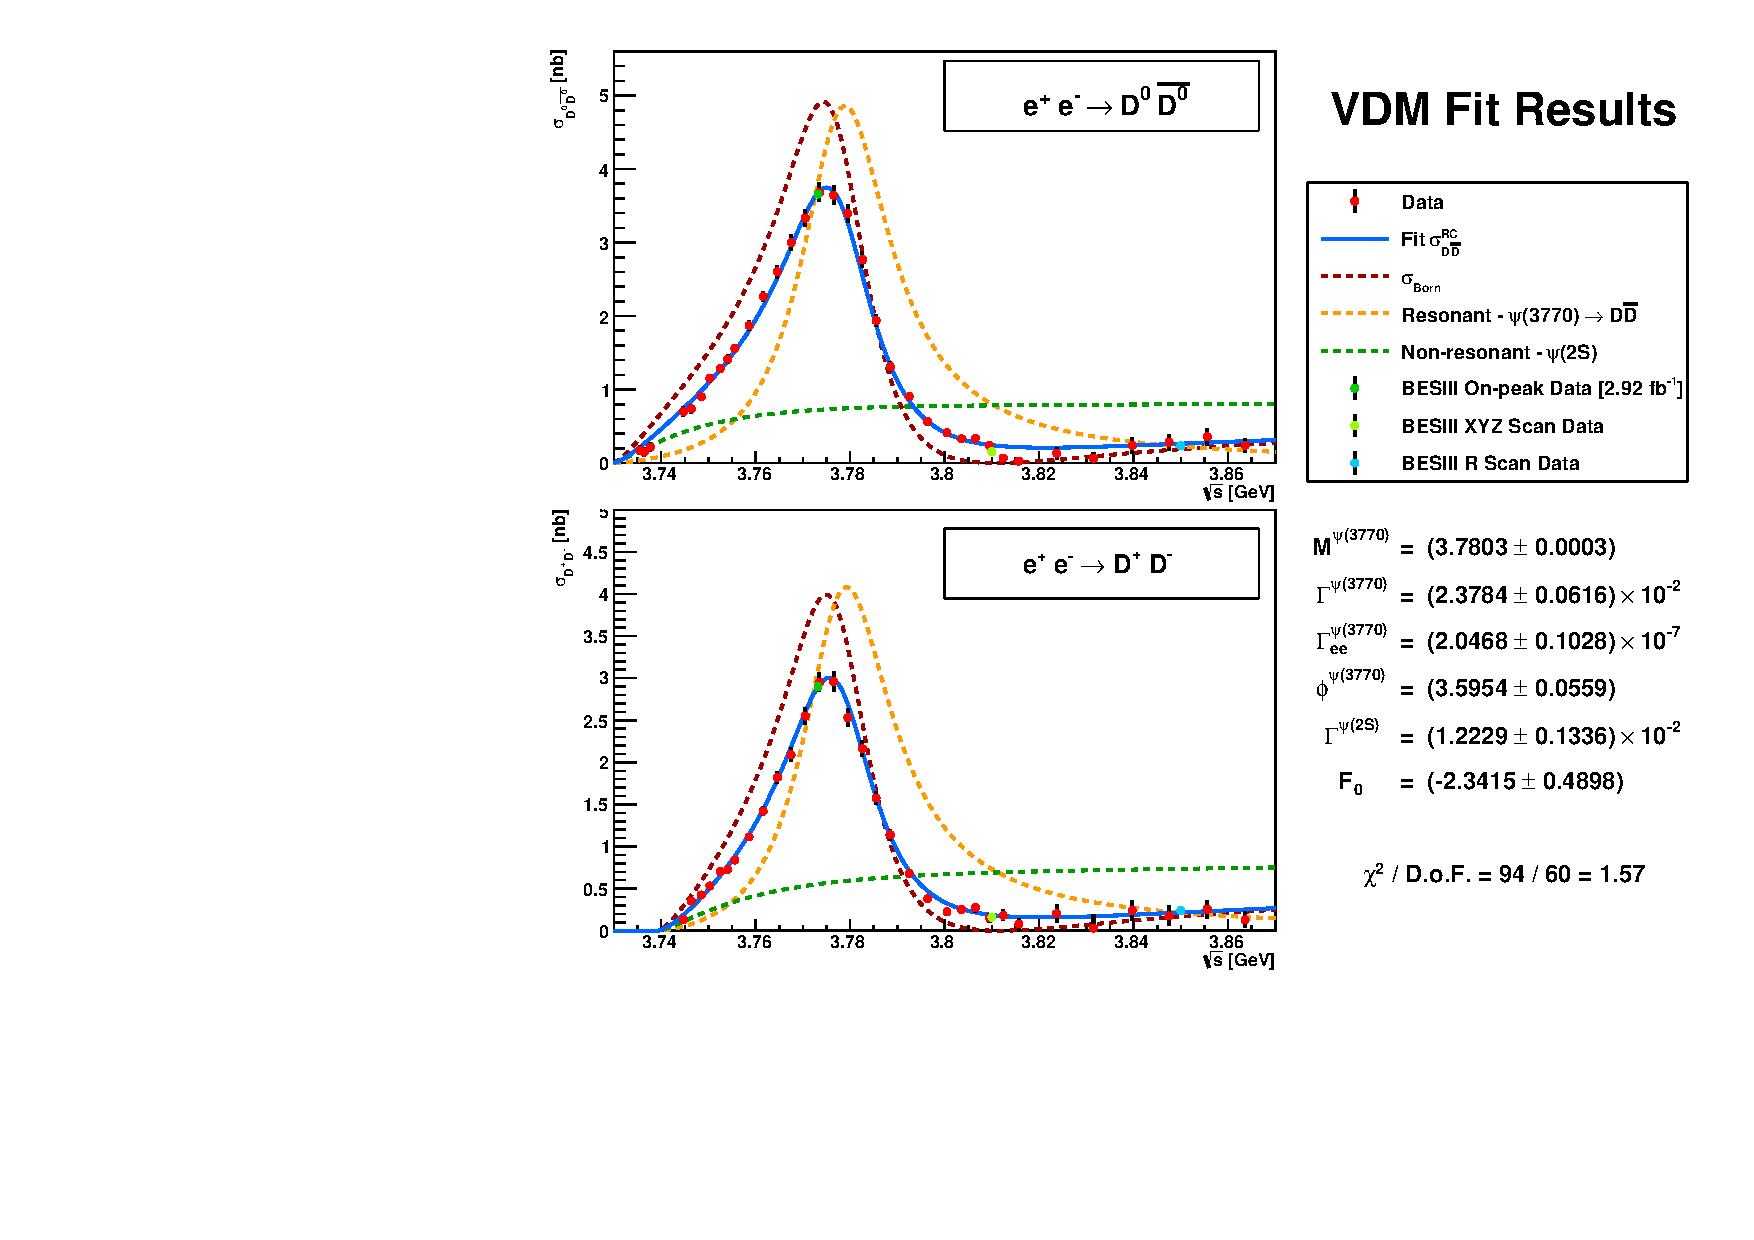
\includegraphics[scale=0.75]{figures/plots/lineshape_vdm_ConExc.pdf}
\caption{The Vector Dominance Model fit results using ConExc.}
{The results for $\DO$ are shown on the top and the results for $\Dp$ are shown on the bottom. The underlying MC shapes for the  $\DDbar$ components were generated with an alternative generator to compare to KKMC.}
\label{fig:ConExc}
\end{figure}



\subsection*{Intermediate Resonances*}
\label{ssec:sys_intermediate_resonances}

In looking at the mode $\DpmodeA$, we also analyzed the contribution of intermediate resonances, like the $\rho^0$.
Using the \SI{2.93}{\invfb} data sample of $\psipp$ events at $\Ecm = \SI{3.773}{\GeV}$, we split the signal region of this mode based on a \SI{1.0}{(\GeV)^2} cut in both the invariant masses of $K \pi$ and $\pi \pi$ separately.
These cuts were chosen to separate the sample into distinctly different regions, as can be seen in \Cref{fig:Kpipi_mass}.
Fitting the signal distributions for each of these subsamples, we found no statistically significant deviations in the measured yields.
From this, we treat variations due to intermediate resonances as negligible.

\begin{figure}[h]
\centering
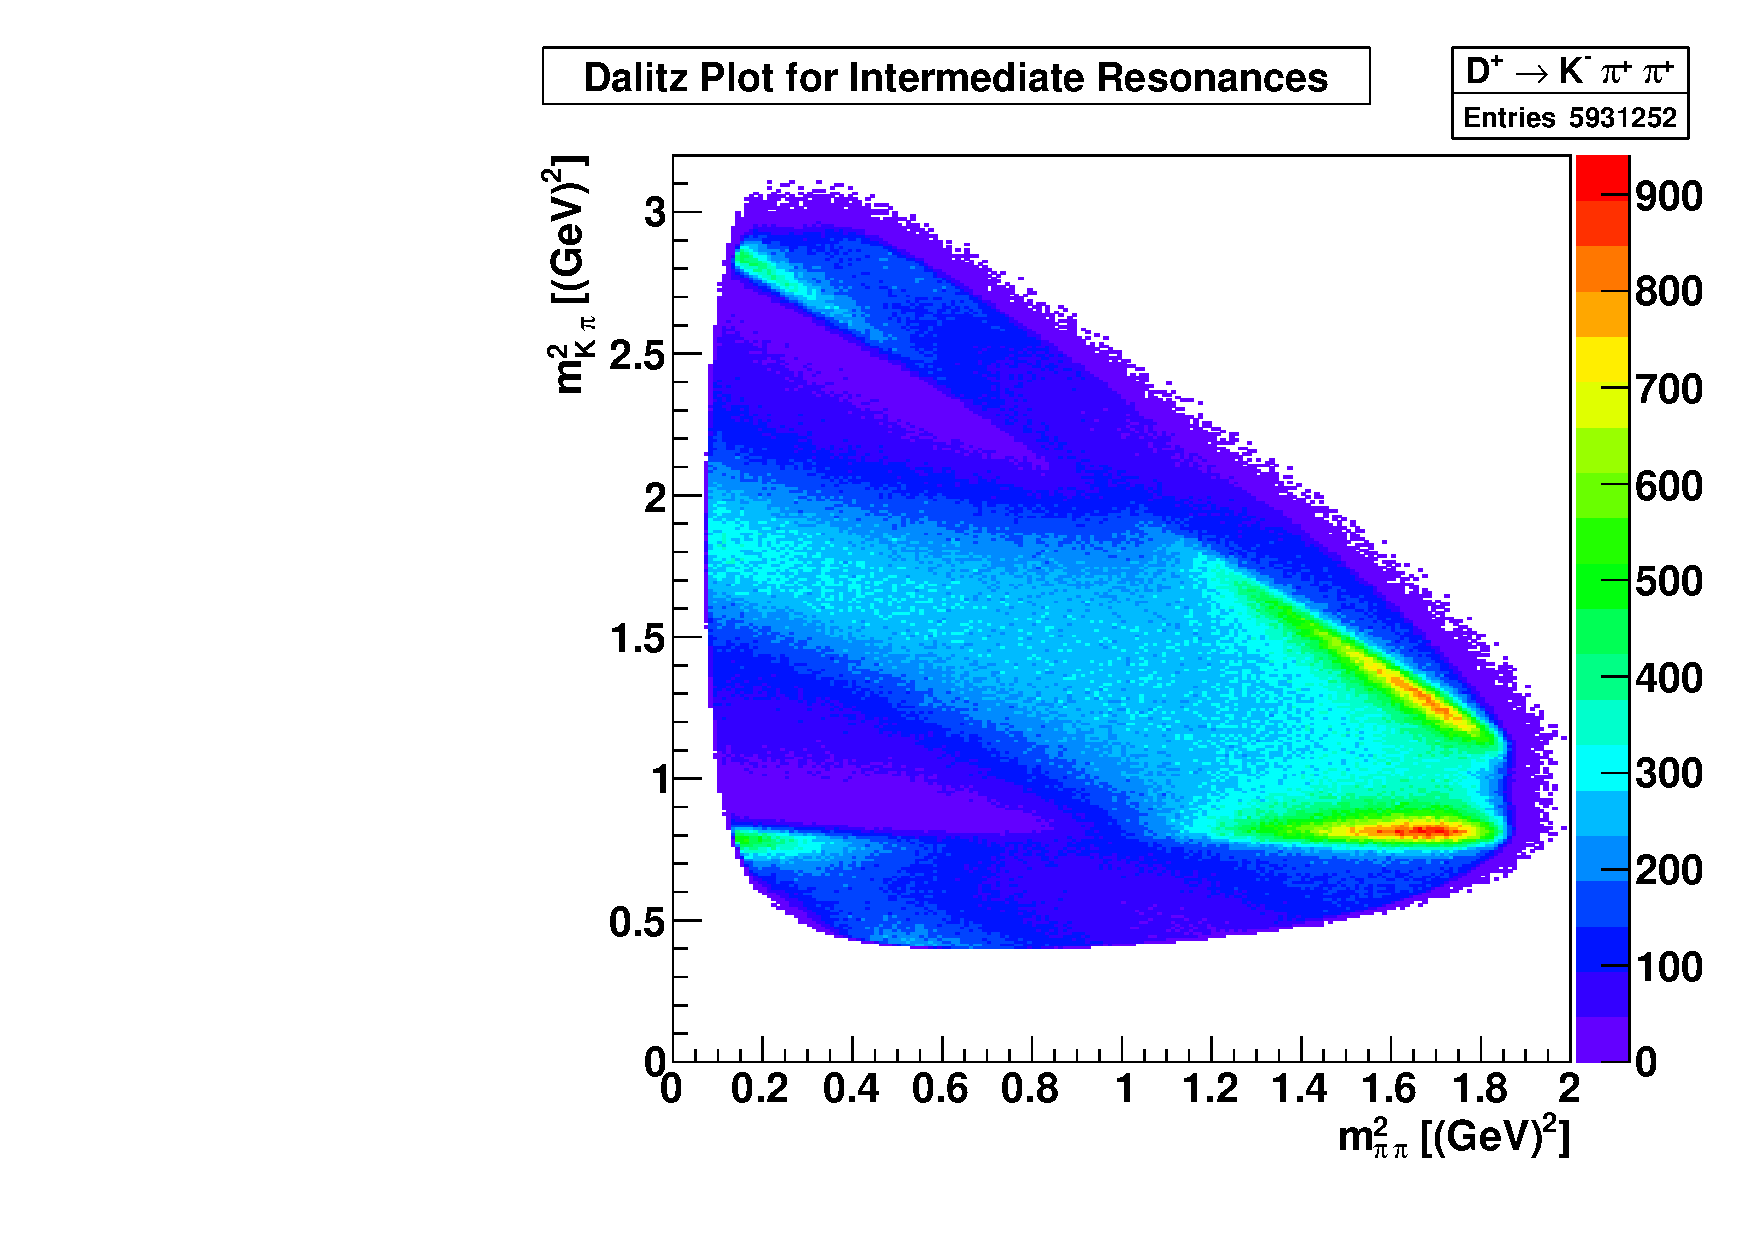
\includegraphics[scale=0.5]{figures/plots/Kpi_vs_pipi_Ecm.pdf}
\caption{The $K \pi$ vs. $\pi \pi$ invariant masses for the mode $\DpmodeA$ with the on-peak $\psipp$ sample.}
\label{fig:Kpipi_mass}
\end{figure}


\subsection*{Form Factor}
\label{ssec:sys_form_factor}

In addition to the systematics described above, there is a significant source of uncertainty coming from the non-resonant form factor used.
Each of the models examined, Exponential and VDM, provided quality fit results for the cross section shapes.
From this, we conservatively assign an uncertainty based on the differences in fit parameters provided by these two methods.
Following the example of KEDR, we treat this as separate from the systematics, and list it as a model uncertainty.









\begin{table}[h]
\centering
\renewcommand\arraystretch{1.0}
\begin{tabular}{c|C{3cm}C{3cm}C{3cm}C{3cm}}
\hline 
Systematic & $\Mpsipp$ [\%] & $\Gpsipp$ [\%] & $\GeepsipptoDD$ [\%] & $\Ppsipp$ [\%] \\
\hline 
Luminosity                          & 0.000 & 0.008 & 0.998 & 0.020 \\
$\Kpm / \pipm$ Tracking             & 0.000 & 0.008 & 3.472 & 0.058 \\
$\piO$ Tracking                     & 0.000 & 0.008 & 1.712 & 0.045 \\
$\Ks$ Tracking                      & 0.000 & 0.004 & 1.278 & 0.036 \\ 
Single Tag Fits                     & 0.000 & 0.004 & 1.186 & 0.022 \\
Meson Radii                         & 0.016 & 2.646 & 3.154 & 1.502 \\
Non-Resonant Form Factor$^\dagger$  & 0.037 & 7.939 & 6.815 & 4.131 \\
\hline
Total [\%]                          & 0.016 & 2.646 & 5.383 & 1.505 \\
Relative Stat. Error [$\sigma$]     & 3.000 & 1.026 & 1.114 & 1.030 \\
\hline
\multicolumn{5}{c}{$^\dagger$The Form Factor is treated as an uncertainty on the model, and is not included in the total systematic error.}
\end{tabular} 
\caption{Systematic uncertainties relative to the measured parameters of the $\psipp$.}
\label{tab:systematics}
\end{table}



\section{Results}
\label{sec:results}


